% Intended LaTeX compiler: xelatex
\documentclass[aspectratio=64,11pt]{beamer}
\usepackage[utf8]{inputenc}
\usepackage{graphicx}
\usepackage{longtable}
\usepackage{wrapfig}
\usepackage{rotating}
\usepackage[normalem]{ulem}
\usepackage{amsmath}
\usepackage{amssymb}
\usepackage{capt-of}
\usepackage{hyperref}
\institute{Università di Siena}
\usepackage{localheader}
\usepackage{tikz}\usetikzlibrary{arrows.meta}
\usepackage{booktabs,tabularx}
\usepackage{setspace}
\usepackage{quoting}
\usepackage[italian]{babel}
\usepackage{fancybox}
\usepackage{icomma}
\newcolumntype{R}{>{\raggedleft\arraybackslash}X}
\newcommand\€{\,\text{€}}
\usetheme{default}
\author{Massimo D'Antoni}
\date{2023-2024}
\title{La tassazione\newline del reddito personale}
\subtitle{Scienza delle Finanze}
\hypersetup{
 pdfauthor={Massimo D'Antoni},
 pdftitle={La tassazione\newline del reddito personale},
 pdflang={Italian}}
\begin{document}

\maketitle

\section{L'imposta personale sul reddito}

%%%%%%%%%%%%%%%%%%%%%%%%%%%%%%%%%%%%%%%%%%%%
\begin{frame}{Il ruolo dell'imposta personale sul reddito}
\begin{itemize}
\item Nelle economie avanzate, l'imposta personale sul reddito riveste un ruolo
centrale
\end{itemize}

\begin{figure}
\centering
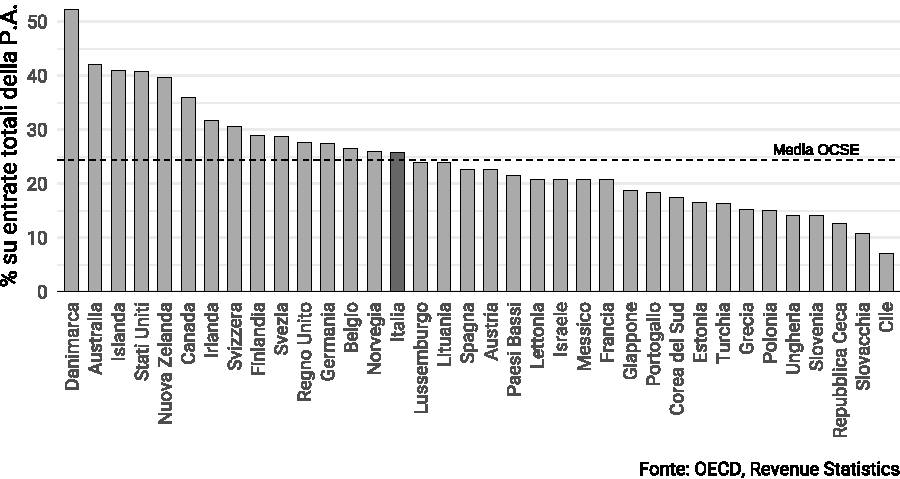
\includegraphics[height=5cm]{./figure/gettito-imposta-personale-OCSE.pdf}
\caption{Gettito delle imposte sui redditi delle persone fisiche in rapporto al totale delle entrate nei paesi OCSE (anno 2019)}
\end{figure}
\end{frame}

%%%%%%%%%%%%%%%%%%%%%%%%%%%%%%%%%%%%%%%%%%%%
\begin{frame}{Dall'imponibile all'imposta}
\begin{figure}
\centering
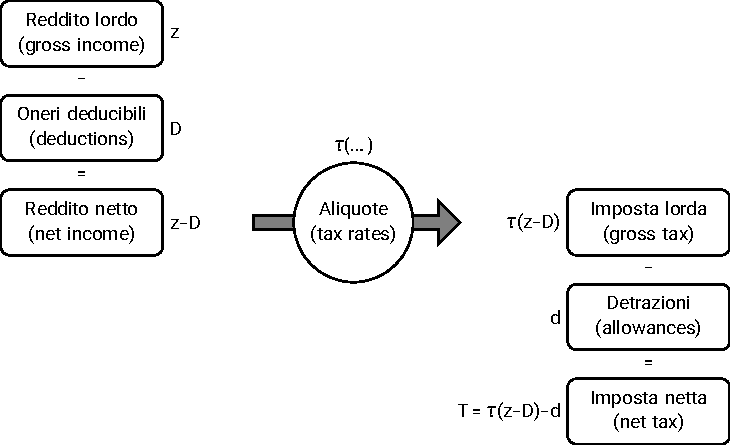
\includegraphics[height=7.5cm]{./figure/da-reddito-a-imposta.pdf}
\end{figure}
\end{frame}


%%%%%%%%%%%%%%%%%%%%%%%%%%%%%%%%%%%%%%%%%%%%
\begin{frame}{Aspetti fondamentali}
\begin{itemize}
\item Le caratteristiche dell'imposta personale sul reddito saranno definite chiarendo:
\begin{itemize}
\item chi tassare
\item cosa tassare (quali redditi)
\item come tassare i redditi
\item quanto tassarli.
\end{itemize}
\item L'obiettivo di distribuire il carico fiscale in modo «equo» può fare riferimento a due criteri:
\begin{itemize}
\item principio del \emph{beneficio}: l'imposta è una sorta di controprestazione per i servizi forniti dallo Stato;
\item principio della \emph{capacità contributiva}: il carico deve essere ripartito in base alla capacità di contribuire, a prescindere dal beneficio.
\end{itemize}
\end{itemize}
\begin{block}{Art. 53 Costituzione}
Tutti  sono  tenuti  a  concorrere  alle spese pubbliche in ragione della loro capacità contributiva.\\[0pt]
Il sistema tributario è informato a criteri di progressività.
\end{block}
\end{frame}

%%%%%%%%%%%%%%%%%%%%%%%%%%%%%%%%%%%%%%%%%%%%
\begin{frame}{Cosa tassare? Un esempio}
\begin{figure}
\centering
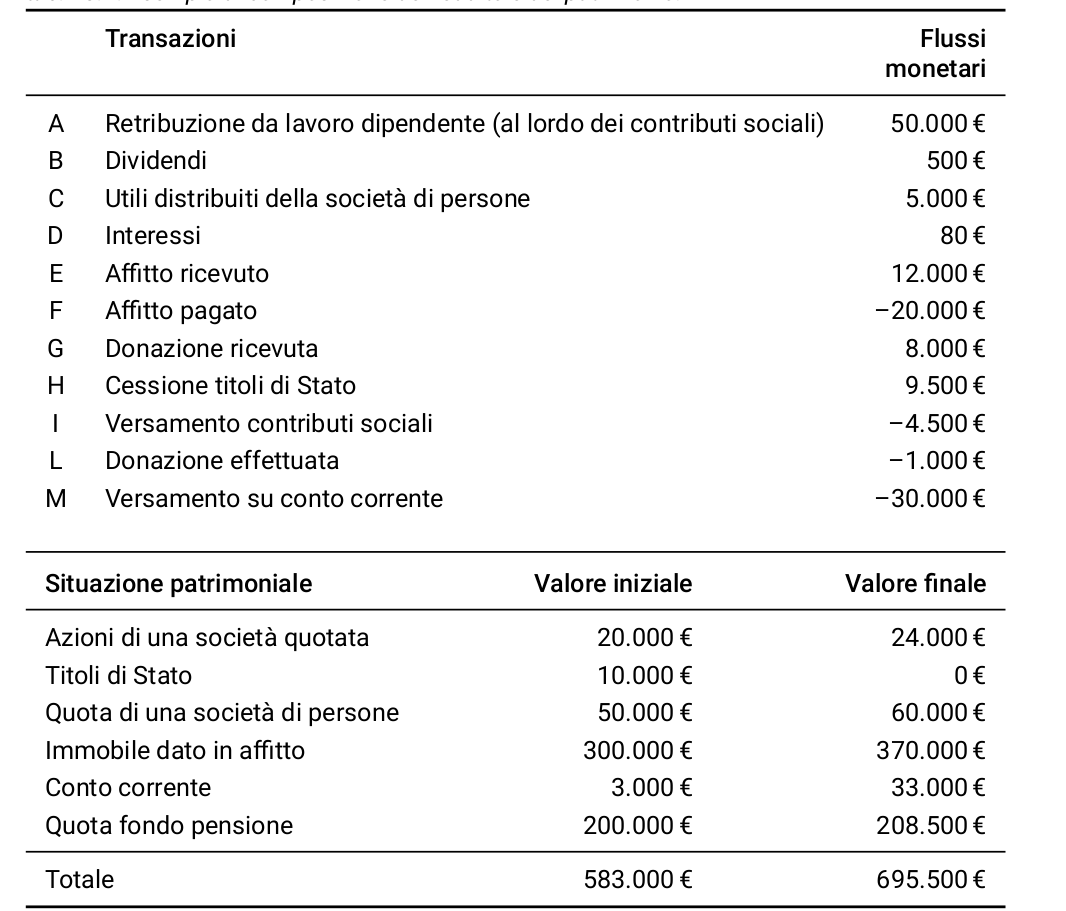
\includegraphics[height=8cm]{./figure/esempio-reddito-patrimonio.png}
\end{figure}
\end{frame}

%%%%%%%%%%%%%%%%%%%%%%%%%%%%%%%%%%%%%%%%%%%%
\begin{frame}{Cosa tassare? Fonte e usi}
\begin{figure}
\centering
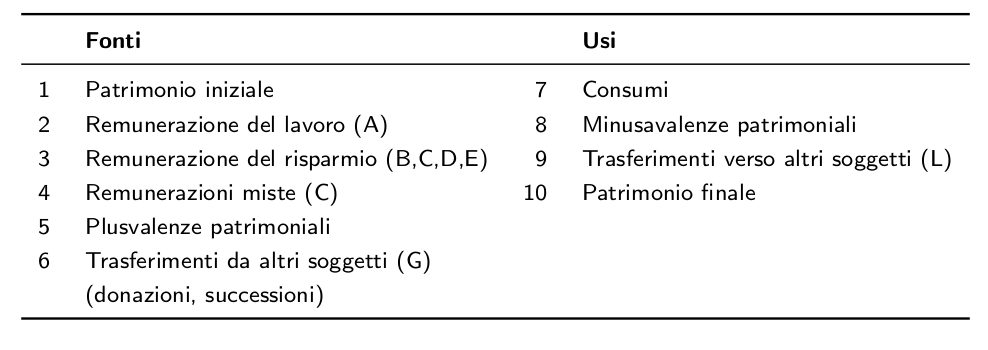
\includegraphics[width=\textwidth]{./figure/esempio-fonti-usi.png}
\end{figure}

\begin{equation*}\label{eq:deltaw}
\begin{split}
\Delta W ={} &\text{risparmio corrente ($2+3+4-7$)} +\\
&{}+\text{plusvalenze nette ($5-8$)}\\
&{}+\text{trasferimenti ricevuti netti ($6-9$)}.
\end{split}
\end{equation*}
\end{frame}

%%%%%%%%%%%%%%%%%%%%%%%%%%%%%%%%%%%%%%%%%%%%
\begin{frame}{Il reddito come prodotto}
De Viti de Marco: i beni e i servizi forniti dallo Stato contribuiscono alla
formazione del prodotto nazionale insieme ai fattori di produzione privati,
lavoro e capitale.

\begin{quoting}
Ogni particella di reddito prodotto contiene la quota-parte di costo, che lo Stato ha sostenuta per la prestazione dei suoi servizi produttori; e poiché l’imposta è il corrispettivo di questo costo, così come il salario è il corrispettivo del lavoro prestato dagli operai, segue che ogni particella di reddito \emph{nasce gravata dal relativo debito tributario}.
\end{quoting}

Le plusvalenze non rientrano in questa nozione di reddito
\end{frame}

%%%%%%%%%%%%%%%%%%%%%%%%%%%%%%%%%%%%%%%%%%%%
\begin{frame}{Tassare le plusvalenze?}
Perché si determinano delle plusvalenze?
\begin{itemize}
\item Inflazione
\item Se si prevede un aumento della produttività del cespite e quindi dei redditi
futuri (es. un brevetto per un'impresa, un'opera pubblica per un immobile).

Inoltre, in molti casi, la plusvalenza corrisponde a una «scommessa», per
cui potrebbero esserci plusvalenze e minusvalenze che si compensano
nell'aggregato.
\item Accantonamento di un reddito in un veicolo finanziario: riduce un reddito
ora per aumentarlo in futuro (es. reinvestimento di un reddito societario
nella società)
\end{itemize}
Tuttavia:
\begin{itemize}
\item la mancata inclusione delle plusvalenze può spingere il contribuente a
eludere indefinitamente la tassazione del capitale trasformando il
rendimento in plusvalenza
\end{itemize}
\end{frame}

%%%%%%%%%%%%%%%%%%%%%%%%%%%%%%%%%%%%%%%%%%%%
\begin{frame}{Il reddito entrata (\emph{comprehensive income})}
\begin{itemize}
\item Definibile come: \alert{il consumo potenziale che il contribuente potrebbe effettuare in un certo periodo senza intaccare la sua ricchezza iniziale.} (Haig \& Simons, vedi anche Musgrave, 1959)
\end{itemize}
\begin{equation*}\label{eq:redentrata}
  \begin{split}
\text{reddito entrata} ={} &\text{consumo effettivo (7)} + \Delta W\\
={}&\text{reddito prodotto ($2+3+4$)}\\
&{}+\text{plusvalenze nette ($5-8$)}\\
&{}+\text{trasferimenti ricevuti netti ($6-9$)}.    
\end{split}
\end{equation*}

\begin{itemize}
\item In particolare, le plusvalenze possono essere tassate
\begin{itemize}
\item alla \alert{maturazione} (ma come determinare il loro ammontare? e se il
contribuente non ha realizzato avrà le risorse per pagare l'imposta?)
\item alla \alert{realizzazione} (ma allora incentivo a non modificare il portafoglio,
effetto \emph{lock in})
\end{itemize}
\end{itemize}
\end{frame}

%%%%%%%%%%%%%%%%%%%%%%%%%%%%%%%%%%%%%%%%%%%%
\begin{frame}{Tassare le plusvalenze alla maturazione?}
\begin{itemize}
\item La tassazione delle plusvalenze alla \alert{maturazione} comporta delle difficoltà:
\begin{itemize}
\item occorre valutare l'incremento di valore, cosa assai difficile se il bene
non viene scambiato su mercati regolamentati;
\item in assenza di una liquidazione del bene, il contribuente potrebbe non
disporre della liquidità necessaria a pagare l'imposta.
\end{itemize}
\item Si optà più spesso per la tassazione alla \alert{realizzazione}. La cessione del
bene ne indica il prezzo e fornisce la liquidità necessaria a pagare
l'imposta. Tuttavia:
\begin{itemize}
\item il contribuente controlla il momento della cessione e può differirla o
realizzarla quando l'aliquota è più bassa.
\item negli USA la regola dello \emph{step-up in basis} esenta dalla
tassazione l'incremento di valore intervenuto nella vita del defunto in
caso di successione \emph{mortis causa};
\item il carico fiscale può essere ridotto/annullato con la creazione di
minusvalenze fittizie;
\item si determina il fenomento del \emph{lock-in};
\item la tassazione alla realizzazione pone problemi in presenza di un'imposta
progressiva.
\end{itemize}
\end{itemize}
\end{frame}


%%%%%%%%%%%%%%%%%%%%%%%%%%%%%%%%%%%%%%%%%%%%
\begin{frame}{Quale reddito tassare? Il reddito consumo o spesa}
\begin{itemize}
\item \alert{Reddito Consumo} o \alert{Reddito spesa} (\emph{expenditure}): la base imponibile
coincide con il consumo effettivo del contribuente nell'anno (Einaudi, 1941;
Kaldor, 1955; Meade, 1978; ma già Hobbes e Mill)
\begin{equation*}\label{eq:redconsumo}
\begin{split}
\text{consumo effettivo (7)} &=\text{reddito entrata} - \Delta W\\
&=\text{reddito prodotto ($2+3+4$)}\\
&\quad{}-\text{risparmio corrente ($2+3+4-7$)}.    
\end{split}
\end{equation*}
\item Tassare la spesa può sembrare molto più complesso che tassare le entrate, ma
non è così
\begin{itemize}
\item L'unica condizione è quella di identificare delle gestioni patrimoniali
(«conti registrati») dalle quali è possibile osservare i flussi in entrata
e uscita.
\item Il reddito spesa sarà così calcolato
\begin{equation*}
 RS_{t}=RP_{t} + (\text{prelievi} - \text{versamenti})
\end{equation*}
\item Equivale ad adottare un criterio di cassa (il corrispettivo nel caso
dell'impresa è la tassazione del \emph{cash flow})
\end{itemize}
\item Vantaggio: non richiede la considerazione esplicita delle plusvalenze
\item Chiaramente si assume in questo caso un'ottica \alert{pluriperiodale}
\end{itemize}
\end{frame}


%%%%%%%%%%%%%%%%%%%%%%%%%%%%%%%%%%%%%%%%%%%%
\begin{frame}{Giustificazioni teoriche del reddito spesa}
\begin{itemize}
\item Già Hobbes (1651):
\begin{quoting}\small
   Per quale ragione colui che molto lavora, risparmia il frutto del suo 
   sudore, consuma poco, dovrebbe pagare di più di colui che vive
   oziosamente, produce poco e spende tutto quel che guadagna...
\end{quoting}
L'idea è che si debba tassare ciò che un individuo «toglie» alle risorse
disponibili con il consumo, non ciò che produce.
\end{itemize}
\end{frame}

%%%%%%%%%%%%%%%%%%%%%%%%%%%%%%%%%%%%%%%%%%%%
\begin{frame}{Giustificazioni del reddito spesa: la «doppia tassazione» del risparmio}
\begin{itemize}
\item J. S. Mill (\emph{Principles of Political Economy}, 1848) avanza l'argomento della \alert{doppia tassazione del risparmio}: se il reddito tassato viene risparmiato, sul rendimento (già tassato) si applica una nuova imposta
\begin{quoting}\small
Tassare la somma investita, e successivamente tassare anche i frutti dell'investimento, significa tassare la stessa porzione dei mezzi del contribuente per due volte. Il capitale e l'interesse non rappresentano due parti distinte che insieme formano le sue risorse, sono la stessa parte contata due volte.
\end{quoting}
\item Esempio: reddito di 1000 €, imposta del 20\%. Il reddito netto di 800 € viene
investito in una rendita perpetua che dà un rendimento del 5\% (pari a 40 €),
su cui si paga l'imposta del 20\%.  Il risparmiatore riceve un flusso di
rendimenti annuo di 32 €, e paga annualmente 8 € di imposte.

Il flusso di imposte future, attualizzato al tasso di rendimento netto del
4\%, è pari a $8€/0,4=160 €$. Il contribuente paga cioè un ulteriore 20\% sul reddito
netto già tassato.
\end{itemize}
\end{frame}

%%%%%%%%%%%%%%%%%%%%%%%%%%%%%%%%%%%%%%%%%%%% 
\begin{frame}{Giustificazioni del reddito spesa: effetti sulle scelte intertemporali}

\begin{itemize}
\item In termini formali, con il reddito entrata abbiamo:  
\begin{gather*}
  c_1=z_1-s-tz_1\\
  c_2=z_2+s(1+r) -t(z_2 +rs)
\end{gather*}
ovvero, sostituendo:
\begin{equation*}
c_1+\frac{c_2}{(1+r)}=
\left[z_1+\frac{z_2}{(1+r)}\right](1-t)-t\frac{rs}{(1+r)}.
\end{equation*}
\item Non viene rispettata l'equità orizzontale tra due contribuenti con diversa
propensione al risparmio.
\item Si determina una distorsione nelle scelte di risparmio, dunque un'allocazione inefficiente del consumo tra i due periodi.
\end{itemize}
\end{frame}

%%%%%%%%%%%%%%%%%%%%%%%%%%%%%%%%%%%%%%%%%%%%
\begin{frame}{Tassare il consumo equivale a esentare il reddito di capitale}
\begin{itemize}
\item Un individuo che percepisce un reddito da lavoro di 30.000 in due periodi e
nel primo periodo risparmia 10.000.
\end{itemize}

\begin{figure}
\centering
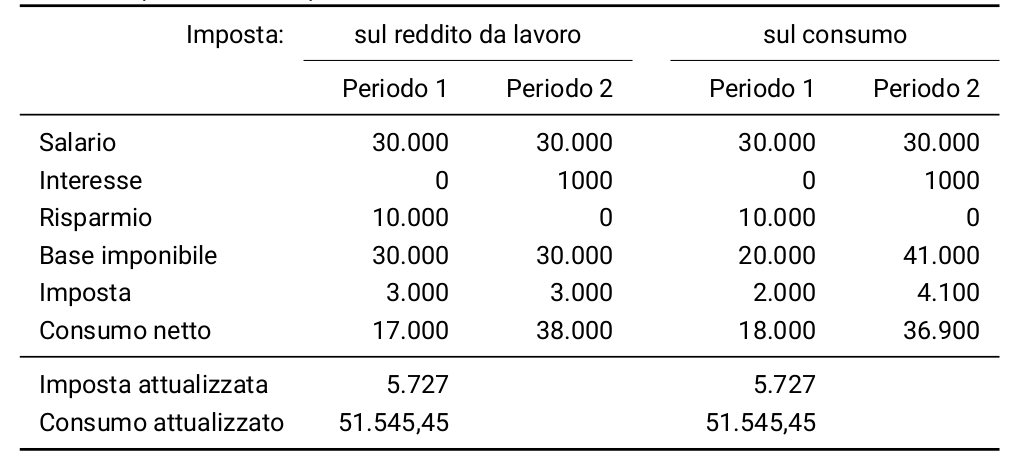
\includegraphics[width=.8\textwidth]{./figure/equivalenza-tassazione-consumo-reddito-da-lavoro.png}
\end{figure}

\begin{itemize}
\item Nota bene: in termini attuariali c'è equivalenza tra le due soluzioni, ma
cambia il profilo temporale dell'imposta.
\end{itemize}
\end{frame}

%%%%%%%%%%%%%%%%%%%%%%%%%%%%%%%%%%%%%%%%%%%%
\begin{frame}{Tassare il consumo equivale a esentare il reddito di capitale /2}
\begin{itemize}
\item Siano $z_1$ e $z_2$ i redditi da lavoro in due periodi
\begin{gather*}
  c_1=(1-t)(z_1-s)\\
  c_2=(1-t)(z_2+s(1+r))
\end{gather*}
da cui:
\begin{equation*}
 c_1+\frac{c_2}{(1+r)}=\left[z_1+\frac{z_2}{(1+r)}\right](1-t)
\end{equation*}
\item La tassazione del consumo equivale, sull'intero orizzonte di vita
dell'individuo, alla tassazione del solo reddito da lavoro (esenzione del
capitale)
\item Con tassazione del capitale avremmo:
\begin{gather*}
  c_1=(1-t)z_1-s\\
  c_2=(1-t)z_2+s(1+(1-t)r)
\end{gather*}
da cui
\begin{equation*}
 c_1+\frac{c_2}{(1+r(1-t))}=\left[z_1+\frac{z_2}{(1+(1-t)r)}\right](1-t)
\end{equation*}
\end{itemize}
\end{frame}

%%%%%%%%%%%%%%%%%%%%%%%%%%%%%%%%%%%%%%%%%%%%
\begin{frame}{I vantaggi della tassazione del consumo in presenza di plusvalenze}
\begin{itemize}
\item Si consideri il caso di un individuo che acquista azioni per 1.000 €. Le
azioni si apprezzano di 100 € nel primo periodo, di altri 200 € nel
secondo.
\item Con il reddito consumo, deduzione di 1.000 € al momento dell'investimento,
mentre al momento del disinvestimento la base imponibile aumenta di
1.300 €.
\item Nel caso del reddito entrata::
\begin{itemize}
\item con la tassazione alla maturazione avremmo il problema di determinare il
valore delle azioni;
\item con la tassazione alla realizzazione vi sarebbe un incentivo a posticipare
la liquidazione.
\end{itemize}
\item Con la tassazione del reddito consumo:
\begin{itemize}
\item non c'è il problema di determinare il valore delle azioni prima della
liquidazione;
\item una ricomposizione del portafoglio (vendita e riacquisto ralla fine del I
periodo) non comporta il pagamento di alcuna imposta, dunque
non c'è effetto \emph{lock-in}.
\end{itemize}
\end{itemize}
\end{frame}

%%%%%%%%%%%%%%%%%%%%%%%%%%%%%%%%%%%%%%%%%%%%
\begin{frame}{Qual è il modello applicato nei paesi OCSE?}
\begin{itemize}
\item Le differenze tra i tre modelli (nozioni di reddito) riguardano il trattamento
del risparmio e delle plusvalenze.
\item In Europa i sistemi fiscali si sono sviluppati a partire dal modello del
reddito prodotto. L'elusione indotta dall'esenzione delle plusvalenze ha
spinto ad assoggettarle a tassazione, con strumenti \emph{ad hoc}.
\item Gli USA, che più coerentemente si erano ispirati al modello del reddito
entrata, includendo le plusvalenze nell'imponibile assoggettato a imposta
progressiva, hanno trovato crescenti difficoltà ad applicare tale modello, e
hanno introdotto forme di tassazione separata.
\item Presenti elementi di reddito consumo per alcune forme di risparmio, in
particolare il risparmio pensionistico.
\item I sistemi si sono spostati verso un \alert{modello duale}, con tassazione
progressiva del reddito da lavoro (e altre componenti), mentre i redditi di
capitale sono assoggettati a imposte proporzionali, più basse.
\end{itemize}
\end{frame}

%%%%%%%%%%%%%%%%%%%%%%%%%%%%%%%%%%%%%%%%%%%%
\begin{frame}{Richiamiamo il diagramma coi flussi}
\begin{figure}
\centering
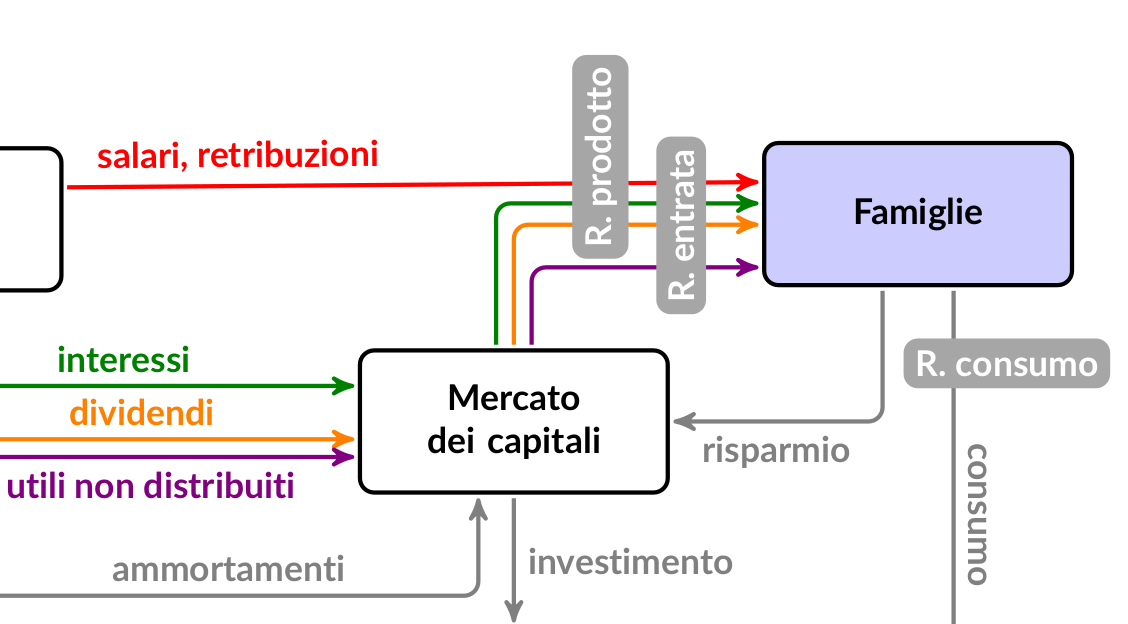
\includegraphics[width=\textwidth]{./figure/flussi-imposte-dettaglio.png}
\end{figure}
\end{frame}

\section{Dall'imponibile all'imposta: la progressività}

%%%%%%%%%%%%%%%%%%%%%%%%%%%%%%%%%%%%%%%%%%%%
\begin{frame}{La progressività del sistema fiscale}
La nostra costituzione recita (art. 53, comma 2)

\begin{center}
Il sistema tributario è informato a criteri di progressività.
\end{center}

\alert{Progressività}: il carico fiscale è proporzionalmente maggiore sugli
  individui più abbienti.
\begin{itemize}
\item progressività \alert{di una singola imposta}: se l'imposta cresce più che
proporzionalmente rispetto alla sua base imponibile
\item progressività \alert{del sistema fiscale nel suo complesso}: può essere realizzato
anche con imposte non progressive, se ad esempio la base imponibile tassata
è concentrata tra gli individui più ricchi
\begin{itemize}
\item un'analisi completa dovrebbe tenere conto anche del modo in cui il gettito
fiscale è utilizzato dal governo: es. per beni consumati in proporzione
maggiore da individui a basso/alto reddito, per ridurre altre imposte (ma
allora l'effetto va calcolato congiuntamente)
\end{itemize}
\end{itemize}
\end{frame}

%%%%%%%%%%%%%%%%%%%%%%%%%%%%%%%%%%%%%%%%%%%%
\begin{frame}{La progressività di un'imposta}
\begin{itemize}
\item Un'imposta è \alert{proporzionale} se il rapporto tra imposta e base imponibile è
costante al variare della base imponibile
\item è \alert{progressiva} (\alert{regressiva}) se l'imposta cresce più (meno) che
proporzionalmente rispetto alla base imponibile
\item In termini di aliquota media: 
\begin{center}
\begin{tabular}{ll}
$T(B)/B$ crescente in $B$ & imposta progressiva\\[0pt]
$T(B)/B$ costante in $B$ & imposta proporzionale\\[0pt]
$T(B)/B$ decrescente in $B$ & imposta regressiva\\[0pt]
\end{tabular}
\end{center}
\item Se l'imposta è progressiva, l'aliquota marginale eccede l'aliquota media:
\begin{equation*}
  \frac{d(T/z)}{dz}=\frac{T'z-T}{z^2}=\frac{1}{z}\left(T'-\frac{T}{z}\right)>0.
\end{equation*}

\item La progressività di un'imposta si ottiene:
\begin{itemize}
\item per \alert{scaglioni}, con aliquota marginale crescente;
\item prevedendo una \alert{deduzione} dall'imponibile o \alert{detrazione} dall'imposta;
\item dagli anni '90 introdotte nel nostro sistema fiscale delle detrazioni
"a scalare", ovvero decrescenti rispetto alla base imponibile.
\end{itemize}
\end{itemize}
\end{frame}

%%%%%%%%%%%%%%%%%%%%%%%%%%%%%%%%%%%%%%%%%%%%
\begin{frame}{Progressività attraverso detrazione o deduzione fissa}
\begin{columns}
\begin{column}{.4\columnwidth}
\small
\begin{itemize}
\item A partire da un'imposta proporzionale, applichiamo una deduzione $D$
  dall'imponibile, oppure una detrazione $d$ dall'imposta:
  \vspace{-3mm}
  \begin{gather*}
    T(B) = t\cdot B - d \\
    T(B)=t\cdot (B-D)
  \end{gather*}
\item Nota bene: se l'aliquota è costante (no scaglioni) e $d=tD$, le due
  soluzioni sono equivalenti.
\item Esempio:
\begin{itemize}
\item aliquota 25\%,
\item deduzione 8.000 €
\item detrazione 2.000 €
\end{itemize}
\end{itemize}
\end{column}

\begin{column}{.6\columnwidth}
\begin{figure}
\centering
\includegraphics[width=\linewidth]{./figure/progressività-ded-detr.pdf}
\end{figure}
\end{column}
\end{columns}
\end{frame}


%%%%%%%%%%%%%%%%%%%%%%%%%%%%%%%%%%%%%%%%%%%%
\begin{frame}{Progressività per scaglioni}
\begin{columns}
\begin{column}{.4\columnwidth}
\small
\begin{itemize}
\item Aliquote marginali $t_1<t_2<\dots t_n$ crescenti, ciascuna applicata alla
parte di reddito imponibile che ricade nel corrispondente scaglione.
\item Esempio:
  \begin{tabular}{lr}
\toprule scaglioni & aliquote \\ \midrule 
0-10.000 & 12\% \\ 
  10.001-30.000 & 20\% \\ 
  oltre 30.000 & 40\% \\
  \bottomrule
\end{tabular}
\end{itemize}
\end{column}

\begin{column}{.6\columnwidth}
\begin{figure}
\centering
\includegraphics[width=\linewidth]{./figure/progressività-esempio.pdf}
\end{figure}
\end{column}
\end{columns}
\end{frame}

%%%%%%%%%%%%%%%%%%%%%%%%%%%%%%%%%%%%%%%%%%%%
\begin{frame}{Progressività per scaglioni in formule}

  \centering
\begin{tikzpicture}
\draw[->, line width=2mm,arrows={-Latex[length=5mm,angle'=90]},
      color=blue!30!white] (1.5,0) to[bend right] (0,-2);
\end{tikzpicture}
%  
  \begin{tabular}[b]{lr}
\toprule scaglioni & aliquote \\ \midrule 
0-10.000 & 12\% \\ 
  10.001-30.000 & 20\% \\ 
  oltre 30.000 & 40\% \\
  \bottomrule
  \end{tabular}
  \hspace{3cm}

  \begin{equation*}
  T(z)=
  \begin{cases}
    12\%\, z & 0\le z\le10.000\\
    12\%\, 10.000 + 20\%\, (z-10.000) & 10.000<z\le30.000\\
    12\%\, 10.000 + 20\%\, (30.000-10.000) + 40\%\,(z-30.000) & z > 30.000
  \end{cases}
\end{equation*}

\begin{columns}
  \begin{column}{.25\textwidth}
    \hfill
\begin{tikzpicture}
\draw[->, line width=2mm,arrows={-Latex[length=5mm,angle'=90]},
      color=blue!30!white] (0,0) to[bend right] (1.5,-1);
\end{tikzpicture}
\end{column}
% 
\begin{column}{.6\textwidth}
  \begin{equation*}
  T(z)=
  \begin{cases}
    12\%\,z & 0\le z\le10.000\\
    1.200 + 20\%\,(z-10.000) & 10.000<z\le30.000\\
    5.200 + 40\%\,(z-30.000) & z > 30.000
  \end{cases}
\end{equation*}
\end{column}
\end{columns}
\end{frame}

%%%%%%%%%%%%%%%%%%%%%%%%%%%%%%%%%%%%%%%%%%%%
\begin{frame}{Evoluzione della struttura degli scaglioni}
\begin{itemize}
\item Tendenza a ridurre il numero degli scaglioni
\end{itemize}

\begin{figure}
\centering
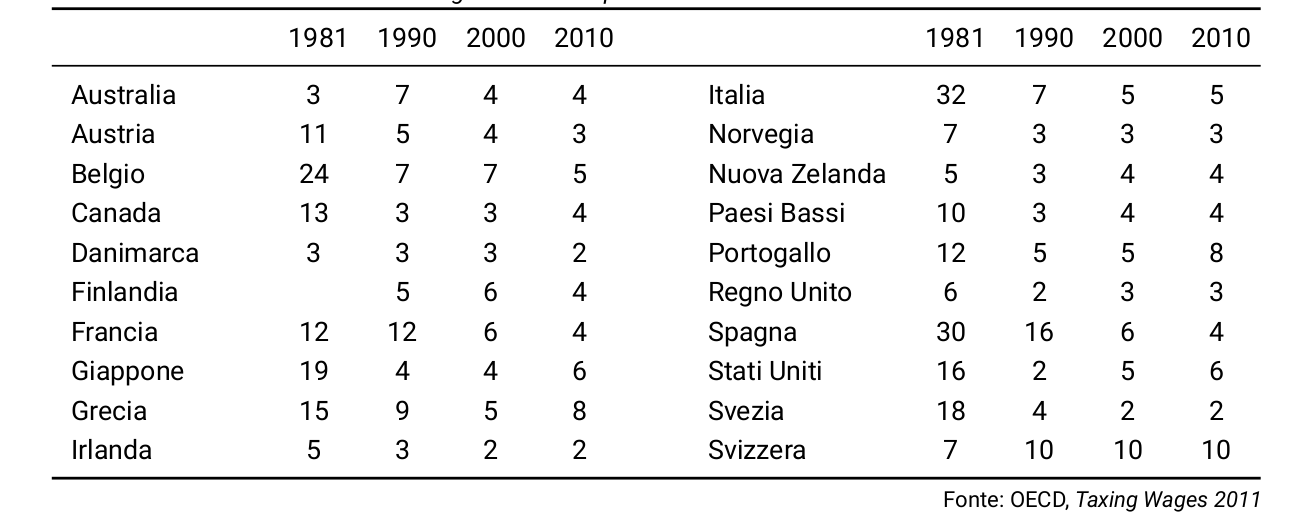
\includegraphics[width=\linewidth]{./figure/evoluzione-numero-scaglioni.png}
\end{figure}
\end{frame}


%%%%%%%%%%%%%%%%%%%%%%%%%%%%%%%%%%%%%%%%%%%%
\begin{frame}{Evoluzione della struttura degli scaglioni/2}
\begin{itemize}
\item Tendenza a ridurre l'aliquota massima
\end{itemize}

\begin{figure}
\centering
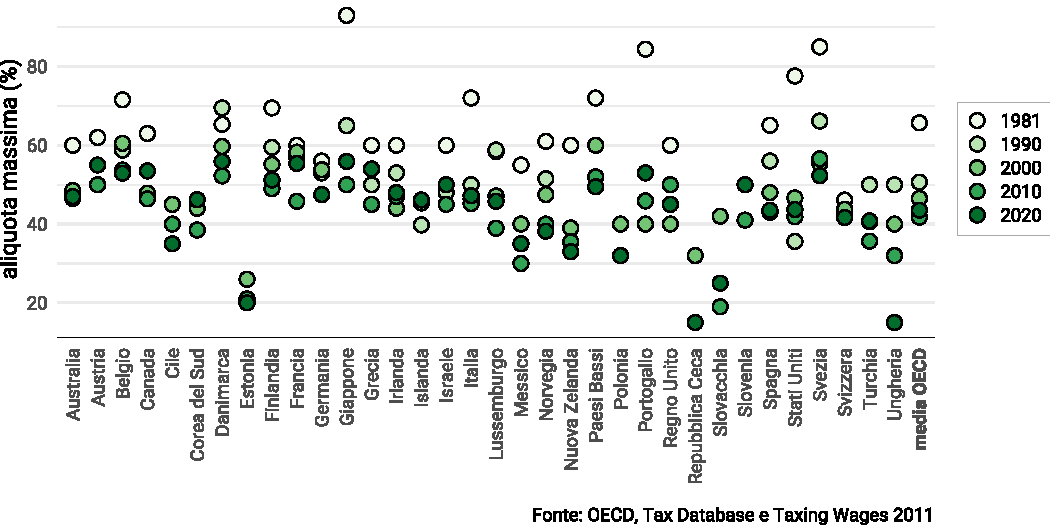
\includegraphics[width=\linewidth]{./figure/top-rates-OCSE-color.pdf}
\end{figure}
\end{frame}

%%%%%%%%%%%%%%%%%%%%%%%%%%%%%%%%%%%%%%%%%%%%
\begin{frame}{Evoluzione degli scaglioni IRPEF}
\begin{figure}
\centering
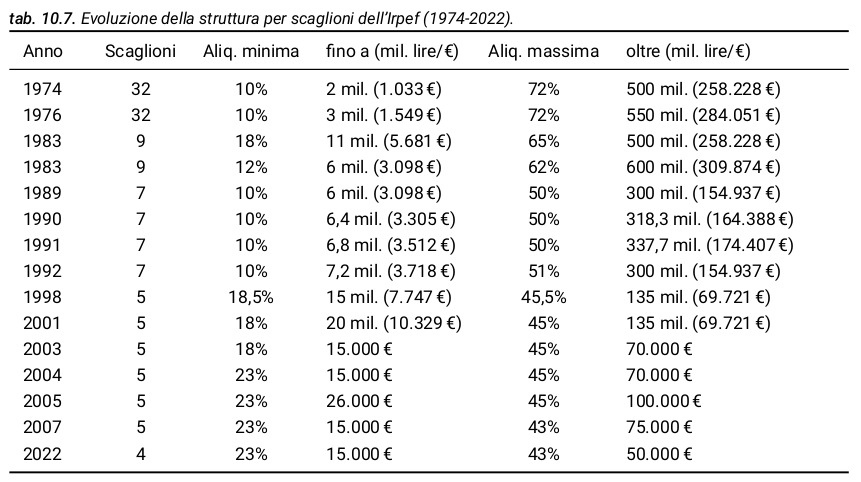
\includegraphics[width=\linewidth]{./figure/evoluzione-scaglioni-IRPEF.png}
\end{figure}
\end{frame}


%%%%%%%%%%%%%%%%%%%%%%%%%%%%%%%%%%%%%%%%%%%%
\begin{frame}{Gli scaglioni IRPEF (dal 2022)}
\begin{figure}
\centering
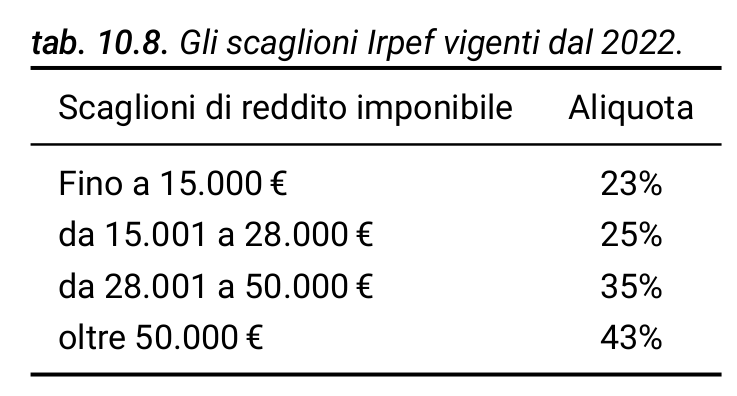
\includegraphics[height=4cm]{./figure/scaglioni-IRPEF-2022.png}
\end{figure}

\begin{equation*}
    \begin{cases}
    23\%\,z & 0\le z\le15.000\\
    3.450 + 25\%\,(z-15.000) & 15.000<z\le28.000\\
    6.700 + 35\%\,(z-15.000) & 28.000<z\le50.000\\
    14.400 + 43\%\,(z-50.000) & z > 50.000
  \end{cases}
\end{equation*}

\end{frame}


%%%%%%%%%%%%%%%%%%%%%%%%%%%%%%%%%%%%%%%%%%%%
\begin{frame}{Combinazione di deduzioni/detrazioni e scaglioni}
\begin{columns}
\begin{column}{.4\columnwidth}
\begin{itemize}
\item In presenza di scaglioni, deduzioni e detrazioni non sono equivalenti.
\item Le deduzioni risultano relativamente più vantaggiose per i redditi più
elevati.
\end{itemize}
\end{column}

\begin{column}{.6\columnwidth}
\begin{figure}
\centering
\includegraphics[width=\linewidth]{./figure/progressività-scaglioni-ded-detr.pdf}
\end{figure}
\end{column}
\end{columns}

\begin{itemize}
\item Una detrazione di 6.000 equivale a una detrazione di 2.400 per i
contribuenti che ricadono nello scaglione massimo (aliquota 40\%).
\item Tuttavia, la stessa deduzione è meno vantaggiosa delle detrazione per i
contribuenti negli scaglioni inferiori.
\end{itemize}
\end{frame}

%%%%%%%%%%%%%%%%%%%%%%%%%%%%%%%%%%%%%%%%%%%%
\begin{frame}{Le detrazioni «a scalare»}
\begin{itemize}
\item A partire dalla fine degli anni Novanta, in luogo delle detrazioni fisse,
sono state introdotte detrazioni "a scalare", il cui ammontare si riduce al
crescere del reddito
\end{itemize}

\begin{block}{}
\begin{figure}
\centering
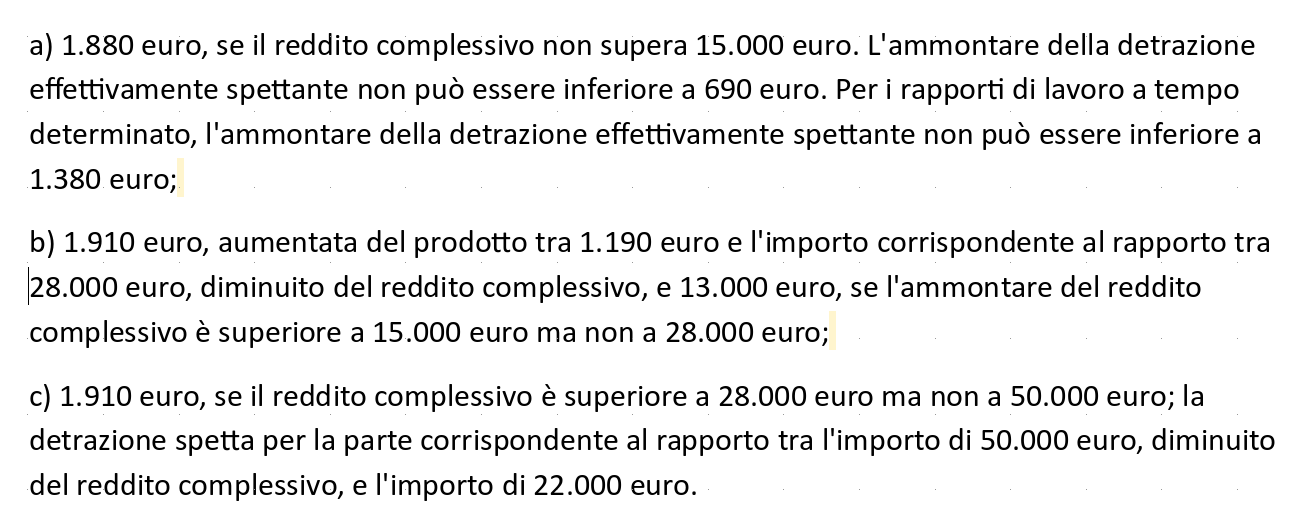
\includegraphics[width=\textwidth]{./figure/detrazione-a-scalare-testo-unico-2022.png}
\end{figure}
\end{block}
\end{frame}


%%%%%%%%%%%%%%%%%%%%%%%%%%%%%%%%%%%%%%%%%%%%
\begin{frame}{La detrazione «a scalare»: un esempio}
\begin{itemize}
\item Ipotizziamo due soli scaglioni
\begin{equation*}
T(z) =
\begin{cases}
  12\%\cdot z & 0\le z\le 30.000\\
  20\%\cdot z + 3.600 & z>30.000.
\end{cases}
\end{equation*}
\item Supponiamo che la detrazione, pari a 720 € per redditi fino a 6.000 €, oltre
questo limite si riduce linearmente fino ad annullarsi in corrispondenza di
30.000 €.
\begin{equation*}
 d(z) =
 \begin{cases}
   720 & z\le 6.000\\
   720\cdot\dfrac{30.000-z}{30.000-6.000} & 6.000<z\le 30.000\\
   0 & z>30.000.
 \end{cases}
 \end{equation*}
\item Per $6.000<z\le 30.000$ la formula si può scrivere come:
$$900 - 720\cdot z/24.000;$$
ogni 1.000 € di reddito la detrazione si riduce di 1/24, ovvero
di 30 €.
\end{itemize}
\end{frame}


%%%%%%%%%%%%%%%%%%%%%%%%%%%%%%%%%%%%%%%%%%%%
\begin{frame}{Le detrazioni «a scalare»}
\begin{figure}
\centering
\includegraphics[width=.75\linewidth]{./figure/progressività-detrazione-a-scalare.pdf}
\end{figure}

\begin{itemize}
\item La riduzione progressiva della detrazione
nell'intervallo tra 6.000 e 30.000 determina un aumento della pendenza, cioè
un aumento dell'aliquota marginale \alert{effettiva}
(in questo caso di $720/24.000=0,03$, cioè del 3\%)
\begin{itemize}
\item una detrazione a scalare è equivalente alla combinazione di (1) una
detrazione fissa e (2) aumento delle aliquote negli scaglioni nei quali la
detrazione decresce
\end{itemize}
\end{itemize}
\end{frame}


%%%%%%%%%%%%%%%%%%%%%%%%%%%%%%%%%%%%%%%%%%%%
\begin{frame}{Progressività, inflazione e \emph{fiscal drag}}
\begin{itemize}
\item In presenza di tassazione progressiva, l'aumento \emph{nominale} dell'imponibile
per effetto dell'inflazione determina un aumento del carico fiscale anche in
assenza di un aumento \emph{reale} del reddito
\item il \emph{fiscal drag} è stato molto rilevante a fini anni '70, con inflazione
>10\%
\item Esempio: 
\begin{itemize}
\item reddito di partenza di 10.000
\item progressività per scaglioni: 20\% fino a 8.000, 30\% oltre
\item nel primo periodo, imposta: $0,2\times 8.000 + 0,3\times 2.000 = 2.200$
\item nel secondo periodo, con inflazione 10\% e reddito nominale è 11.000, il
reddito reale non è variato.
\item L'imposta è: $0,2\times 8.000 + 0,3\times 3.000 = 2.500$. \\[0pt]
L'aliquota media è cresciuta dal 22\% al 22,7\%, a parità di reddito reale
\end{itemize}
\item \emph{Soluzione 1}: indicizzare gli scaglioni, le detrazioni ecc.
\item \emph{Soluzione 2}: si riporta il reddito corrente all'anno base, depurandolo
dall'inflazione, si applica la struttura delle aliquote ecc. Una volta
calcolata l'aliquota media la si applica al reddito corrente
\end{itemize}
\end{frame}

%%%%%%%%%%%%%%%%%%%%%%%%%%%%%%%%%%%%%%%%%%%%
\begin{frame}{Chi tassare? La scelta dell'unità impositiva}
In presenza di un'imposta progressiva ciascuna soluzione presenta dei
vantaggi/svantaggi:
\begin{columns}
\begin{column}{.5\columnwidth}
\begin{block}{LA FAMIGLIA.}
\small
\begin{itemize}
\item Un migliore indicatore della vera capacità contributiva
\item Neutralità rispetto all'intestazione del reddito: elimina l'incentivo a
intestare reddito al coniuge con reddito minore.
\item Neutralità rispetto alla composizione della famiglia a parità di reddito
complessivo: nessuna penalizzazione per le famiglie monoreddito.
\end{itemize}
\end{block}
\end{column}

\begin{column}{.5\columnwidth}
\begin{block}{L'INDIVIDUO.}
\small
\begin{itemize}
\item Neutralità rispetto alla decisione di formare una famiglia, laddove la base
familiare penalizza la costituzione di un vincolo familiare.
\item Neutralità rispetto alle decisioni di offerta del lavoro: con la base
familiare ci possono essere effetti negativi sull'offerta del lavoro
femminile (aliquota marginale più elevata per il titolare di reddito
inferiore).
\end{itemize}
\end{block}
\end{column}
\end{columns}
\end{frame}

%%%%%%%%%%%%%%%%%%%%%%%%%%%%%%%%%%%%%%%%%%%%
\begin{frame}{La tassazione su base familiare con imposizione progressiva}
\begin{itemize}
\item Due coniugi con redditi $z_1$ e $z_2$ (diversi tra loro) assoggettati a
imposta descritta dalla funzione $T(z)$.
\item Nulla cambia se l'imposta è proporzionale, ovvero $T(z)=tz$:
\begin{equation*}
  T(z_1+z_2)=t(z_1+z_2)=tz_1+tz_2)=T(z_1)+T(z_2).
\end{equation*}
\item Se l'imposta $T(z)$ è progressiva:
\begin{equation*}
  T(z_1+z_2)=\frac{T(z_1+z_2)}{z_1+z_2}(z_1+z_2) >
  \frac{T(z_1)}{z_1} z_1 + \frac{T(z_2)}{z_2} z_2 = T(z_1)+T(z_2)
\end{equation*}
in quanto la progressività di $T(z)$ implica che $\frac{T(z_1+z_2)}{z_1+z_2}>\frac{T(z_i)}{z_i}$.
\end{itemize}

\begin{block}{}
\small
Nel 1976 la C. Costituzionale dichiarò illegittima, in quanto discriminatoria
tra i due coniugi e penalizzante per le coppie unite in matrimonio rispetto a quelle di fatto, l'applicazione dell'Irpef su base familiare prevista dalla riforma del 1973, laddove si stabiliva che ai fini del pagamento dell'imposta i redditi della moglie dovessero essere imputati al marito.
\end{block}
\end{frame}

%%%%%%%%%%%%%%%%%%%%%%%%%%%%%%%%%%%%%%%%%%%%
\begin{frame}{Lo \emph{splitting}}
\begin{itemize}
\item Con lo \alert{\emph{splitting}}, opzione consentita ai coniugi in Germania, a
ciascun coniuge si attribuisce un reddito pari al reddito medio:
\begin{equation*}
  \bar{z}=\frac{z_{1}+z_{2}}{2}
\end{equation*}
\item Assumiamo che $z_{1}>z_{2}$ e che l'aliquota marginale sia crescente, per
cui,
\begin{equation*}
  \frac{T(z_{1})-T(\bar z)}{z_{1}-\bar{z}}
  >\frac{T(\bar{z})-T(z_{2})}{\bar{z}-z_{2}}
  \quad\text{}
\end{equation*}
visto che $z_{1}-\bar{z}=\bar{z}-z_{2}$, abbiamo che
\begin{equation*}
  T(z_{1})-T(\bar{z})>T(\bar{z})-T(z_{2})\quad\implies\quad
  2T(\bar{z})<T(z_{1})+T(z_{2}).
\end{equation*}
con lo \emph{splitting} l'imposta pagata complessivamente dai due coniugi risulta
dunque inferiore rispetto a quanto pagherebbero individualmente.
\item Notiamo tuttavia che per il coniuge con reddito più basso l'aliquota
marginale sarà maggiore rispetto al caso di tassazione individuale. La sua
offerta di lavoro sarà maggiormente disincentivata.
\end{itemize}
\end{frame}

%%%%%%%%%%%%%%%%%%%%%%%%%%%%%%%%%%%%%%%%%%%%
\begin{frame}{Il quoziente familiare}
\begin{itemize}
\item Il sistema del \alert{quoziente familiare} (adottato in Francia) segue la stessa
logica dello \emph{splitting}, ma tiene conto anche della presenza di altri
familiari a carico.
\item Al reddito complessivo della famiglia si applica un quoziente $q$ deteminato
in base alla composizione familiare: $q$ vale 2 per una coppia, viene aumentato di 0,5 per ciascun figlio per i primi 2 figli e di 1 per ciascun figlio oltre il secondo.
\item L'imposta da pagare a livello familiare è data da:
\begin{equation*}
  q\cdot T\left( \frac{\sum_{h}Y_{h}}{q} \right)
\end{equation*}
\item Esempio: una famiglia con un unico contribuente con reddito 100.000 €, una
moglie e 4 figli. Il quoziente è $q=5$. Invece di applicare a 100.000 €
l'aliquota media corrispondente a tale livello, vi si applicherà l'aliquota
media (ben più bassa) corrispondente a 20.000 €
\item Nota bene: a parità di numerosità della famiglia, il vantaggio è tanto
maggiore quanto più alto è il reddito.
\end{itemize}
\end{frame}

\section{L'Imposta sul Reddito delle Persone Fisiche (IRPEF)}


%%%%%%%%%%%%%%%%%%%%%%%%%%%%%%%%%%%%%%%%%%%%
\begin{frame}{L'IRPEF: soggetti passivi e base imponibile}
\begin{columns}
\begin{column}{.5\columnwidth}
\begin{block}{IRPEF}
Un'imposta personale, progressiva, che si applica:
\begin{itemize}
\item al complesso dei redditi posseduti (all'interno o all'esterno dello Stato)
per gli individui residenti;
\item ai redditi prodotti nel territorio dello Stato per i non residenti.
\end{itemize}
\end{block}
\end{column}

\begin{column}{.5\columnwidth}
Si determina seguendo il cosiddetto «modello delle fonti»:
\begin{center}
\begin{tabular}{l}
redditi fondiari\\[0pt]
$+$ redditi di capitale (dividendi)\\[0pt]
$+$ redditi da lavoro autonomo\\[0pt]
$+$ redditi da lavoro dipendente\\[0pt]
$+$ reddidi di impresa\\[0pt]
$+$ redditi diversi\\[0pt]
$=$ \alert{reddito complessivo}: $Y$\\[0pt]
$-$ deduzioni: $D$\\[0pt]
$=$ reddito imponibile: $Y-D$\\[0pt]
(applicazione struttura aliquote)\\[0pt]
$=$ imposta lorda: $t(Y-D)$\\[0pt]
$-$ detrazioni: $d$\\[0pt]
$=$ \alert{imposta netta}: $T=t(Y-D)-d$\\[0pt]
\end{tabular}
\end{center}
\end{column}
\end{columns}
\end{frame}



%%%%%%%%%%%%%%%%%%%%%%%%%%%%%%%%%%%%%%%%%%%%
\begin{frame}{1. I redditi fondiari}
Nell'ambito dei redditi fondiari distinguiamo tra:
\begin{itemize}
\item \alert{redditi da terreni}
\begin{itemize}
\item redditi \alert{dominicali} (la "rendita fondiaria")
\item redditi \alert{agrari} (il profitto dell'imprenditore agricolo, che svolge
addività di coltivazione, silvicoltura, allevamento e attività connesse)
inclusi redditi delle costruzioni rurali utilizzate nell'ambito di queste
attività
\end{itemize}
\item \alert{redditi da fabbricati} (N.B. esclusi quelli rurali e quelli di cui sono titolari
imprese commerciali)
\end{itemize}

\begin{columns}
  \begin{column}{.5\textwidth}
La base imponibile è determinata
\begin{itemize}
\item dal \alert{canone di affitto o di locazione}, per i terreni in affitto e gli immobili
in locazione
\item dalla \alert{rendita catastale} in tutti gli altri casi (reddito ``normale'')
\end{itemize}
\end{column}
\begin{column}{.5\textwidth}
\begin{block}{}
\small
L'adozione, invece del reddito effettivo, di un criterio di \alert{reddito
normale}, ovvero un reddito medio rispetto ad attività omogenee e su un
orizzonte più lungo, si giustifica: (1) per la semplicità amministrativa; (2) per
la presenza di componenti di reddito non monetario; (3) per la variabilità del
reddito nel tempo; (4) per l'arbitrarietà del periodo di imposta.
\end{block}
\end{column}
\end{columns}
\end{frame}
%%%%%%%%%%%%%%%%%%%%%%%%%%%%%%%%%%%%%%%%%%%%
\begin{frame}{1. Redditi fondiari}
\begin{itemize}
\item Dal 2017 è prevista l'esenzione per i redditi dominicali e agrari
(inizialmente prevista solo fino al 2019, ma prorogata di anno in anno)
\item Dal 2012 i redditi dominicali e quelli da fabbricati sono assoggettati a
Irpef solo se locati.
\item Se non locati e diversi da abitazione principale, l'Irpef è assorbita
dall'Imu, Imposta Municipale Unica.
\begin{itemize}
\item Eccezione: gli immobili non locati nel Comune dell'abitazione principale,
che sono inclusi al 50\% nell'Irpef della rendita (+5\%) maggiorata di 1/3
\end{itemize}
\item Il reddito catastale dell'abitazione principale concorre al reddito
complessivo Irpef ma viene integralmente dedotto ai fini della
determinazione dell'imposta
\begin{itemize}
\item Eccezione: abitazioni «di lusso», cat. A1, A8 e A9.
\end{itemize}
\end{itemize}
\end{frame}

%%%%%%%%%%%%%%%%%%%%%%%%%%%%%%%%%%%%%%%%%%%%
\begin{frame}{1. Redditi fondiari /2}
\begin{itemize}
\item Nel caso dei redditi da fabbricati locati:
\begin{itemize}
\item il canone di locazione ovvero, se più elevata, dalla rendita catastale
rivalutata del 5\%, concorre all'imponibile IRPEF.

Il canone è ridotto forfetariamente del 5\% per tenere conto di costi di
manutenzione e gestione (ulteriore riduzione del 30\% se "canone
convenzionale" in aree ad alta densità abitativa)
\item è possibile \alert{optare} per un'imposta \alert{cedolare secca sostitutiva} del 21\%
(applicata al canone o alla rendita rivalutata). L'aliquota è ridotta al
10\% nel caso di contratti stipulati con "canone convenzionale".
\end{itemize}
\end{itemize}

\begin{block}{È equo escludere l'abitazione principale dalla tassazione?}
Il reddito dell'abitazione principale è escluso dall'IRPEF e non è assoggettato all'IMU.

L'argomento per cui la casa di abitazione rappresenta un "bene primario" trascura il fatto che il valore della casa può essere molto diverso tra contribuenti e pone un problema di equità orizzontale tra contribuenti proprietari e contribuenti che abitano in immobile in locazione.
\end{block}
\end{frame}

%%%%%%%%%%%%%%%%%%%%%%%%%%%%%%%%%%%%%%%%%%%%
\begin{frame}{2. I redditi di capitale}
\begin{itemize}
\item \alert{Redditi di capitale}: redditi derivanti dall’impiego di capitale
finanziario con l'eccezione di quelli \alert{conseguiti nell’esercizio di impresa}
(ricompresi tra i redditi di impresa) e di \alert{plusvalenze} e proventi dei
prodotti \alert{derivati} (se la prestazione è "in dipendenza di eventi incerti",
sono classificati come redditi diversi).
\item In pratica, sono soggetti a Irpef soltanto i \alert{dividendi} da società di
capitali se questa è residente in un "paradiso fiscale"
\item In tutti gli altri casi si applicano \alert{imposte sostitutive} con aliquota del
26\%, del 12,5\% (titoli pubblici) e del 20\% (risparmio previdenziale)
\item Il fatto che i redditi di capitale non possano assumere valori negativi
implica che:
\begin{itemize}
\item il nostro sistema non consente in generale agli individui la deduzione degli
interessi passivi (consentita solo per mutui agrari o acquisto abitazione principale);
\item non possibile dedurre interessi negativi;
\item non possibile compensare una perdita di un fondo comune (classificata come
minusvalenza) con un guadagno corrente o futuro dello stesso o altri fondi
(considerato reddito di capitale).
\end{itemize}
\end{itemize}
\end{frame}

%%%%%%%%%%%%%%%%%%%%%%%%%%%%%%%%%%%%%%%%%%%%
\begin{frame}{3. I redditi da lavoro dipendente}
\begin{itemize}
\item \alert{Redditi da lavoro dipendente e pensione}: includono ogni forma di compenso al
lavoratore dipendente nonché le pensioni e i proventi conseguiti in
sostituzione di redditi da lavoro (indennità di disoccupazione, di mobilità
ecc.).
\item Sono \emph{assimilati} ai redditi da lavoro dipendente le rendite dei fondi
pensione, le rendite delle polizze vita, nonché altri compensi che non
rientrano nell'esercizio di arte o professione (compresi compensi a figure
di lavoro occasionali o precarie)
\item Sono inclusi i \alert{fringe benefit} (es. auto aziendali)
\item Sono calcolati secondo un \alert{criterio di cassa} e al \alert{lordo} dei costi di
produzione sostenuti dal contribuente (vedi però maggiore detrazione).
\item I datori di lavoro operano da \emph{sostituti di imposta} con \emph{obbligo di
rivalsa} sul contribuente (operano cioè una ritenuta d'acconto che versano
all'erario). Ciò rende tali redditi facili da accertare.
\begin{itemize}
\item Vantaggio per il contribuente: in molti casi superfluo effettuare la
dichiarazione
\item Dal 2008 i premi di risultato sono esclusi e assoggettati a imposta
sostitutiva del 10\%: erosione della base imponibile dell'imposta progressiva
\end{itemize}
\end{itemize}
\end{frame}

%%%%%%%%%%%%%%%%%%%%%%%%%%%%%%%%%%%%%%%%%%%%
\begin{frame}{3. I redditi da lavoro dipendente (i \emph{fringe benefit})}
\begin{itemize}
\item Problemi particolari posti da remunerazione non monetaria, es. auto
aziendale o altro \emph{fringe benefit}
\item regola generale: conteggiati al valore normale praticato dall'azienda
\item Per gli \alert{autoveicoli} si pone il problema di distinguere tra uso esclusivo
per l'azienda o uso promiscuo. In questo secondo caso:
\begin{itemize}
\item per l'impresa deducibilità dei costi (di acquisto, manutenzione ecx.) al 70\%
\item nel reddito del dipendente, reddito calcolato come valore equivalente a
percorrenza annua convenzionale (30\% di 15.000 km, calcolo con tabelle
Aci)
\end{itemize}
\item per i fabbricati in locazione a condizioni agevolate, la differenza tra
rendita catastale e quanto corrisposto dal dipendente
\item le indennità di trasferta (se non rimborsate analiticamente) sono
considerate reddito per la parte che eccede un limite fissato per legge
\end{itemize}
Complessità della normativa e criteri forfetari per limitare la possibilità di
elusione fiscale
\end{frame}
%%%%%%%%%%%%%%%%%%%%%%%%%%%%%%%%%%%%%%%%%%%%
\begin{frame}{4. redditi da lavoro autonomo}
\begin{itemize}
\item \alert{Redditi di lavoro autonomo:} Redditi che derivano dall’esercizio abituale
(anche se non esclusivo) di arti e professioni (assenza del vincolo di
subordinazione), dall’utilizzazione economica di opere dell’ingegno e di
brevetti industriali (se non conseguiti nell’esercizio di impresa).
\end{itemize}
Due regimi:
\begin{enumerate}
\item \emph{Esercenti arti o professioni con ricavi annui superiori a 85.000 euro}. Il
reddito imponibile, determinato con \alert{criterio di cassa}, è un \alert{reddito
netto}. Sono ammesse in deduzione le spese di produzione del reddito, con
alcune limitazioni finalizzate a evitare abusi:
\begin{itemize}
\item limiti alla possibilità di ammortamento dei beni strumentali
\item deducibilità al 50\% per beni con uso promiscuo
\item non ammessa deducibilità dei compensi al coniuge o ai figli
\item limiti alla deducibilità delle spese di rappresentanza, alberghi ecc.
\item Consentita contabilità semplificata per redditi entro 309.874 euro
\end{itemize}
L'accertamento di questi redditi da sempre considerato difficile.
Ove possibile chi corrisponde un compenso è tenuto ad operare da sostituto
di imposta, applicando una ritenuta d'acconto del 20\%.
\end{enumerate}
\end{frame}

%%%%%%%%%%%%%%%%%%%%%%%%%%%%%%%%%%%%%%%%%%%%
\begin{frame}{4. redditi da lavoro autonomo /2}
\begin{enumerate}
\setcounter{enumi}{1}
\item \emph{Esercenti arti o professioni con ricavi annui fino a 85.000
euro}. Regime forfetario (c.d. \emph{flat tax}) che prevede una definizione
forfetaria del reddito, l'applicazione di un'imposta sostitutiva del 15\%,
l'esenzione da altre imposte (IRAP, addizionali) e l'esenzione IVA dei beni
e servizi prodotti.
\begin{itemize}
\item Il reddito si determina applicando ai ricavi, al netto dei contributi
previdenziali, un coefficiente di redditività che dipende dall'attività
svolta;
\item Alcune limitazioni: nell'anno precedente non devono essere stati
percepiti, nell'ambito di rapporti tuttora esistenti, redditi da
lavoro/pensione eccedenti i 30.000 euro; non devono essere stati
corrisposti compensi a dipendenti eccedenti i 20.000 euro
\end{itemize}
Problemi: 
\begin{itemize}
\item rischio di elusione (false partite IVA)
\item disincentivo alla crescita
\end{itemize}
\end{enumerate}
\begin{block}{}
\small
Disciplina mutevole: regime forfetario introdotto nel 2014 per redditi
"minimi" con limite 30.000 euro. La L. Bilancio 2019 ha esteso il limite a
65.000 e ha introdotto un secondo regime forfetario (successivamente abolito)
con aliquota 20\% per i redditi fino a 100.000. A partire dal 2023 il nuovo
limite è 85.000.
\end{block}
\end{frame}

%%%%%%%%%%%%%%%%%%%%%%%%%%%%%%%%%%%%%%%%%%%%
\begin{frame}{5. redditi di impresa}
\begin{itemize}
\item \alert{Redditi di impresa:} Reddito derivante dall’esercizio di imprese
commerciali in forma individuale o associata (società di persone e \emph{in
alcuni casi} società a responsabilità limitata).
\item I criteri di determinazione del reddito di impresa sono comuni sia all’IRPEF
che all’IRES.  Il reddito di impresa coincide con l'utile, con alcune
variazioni rispetto alla normativa civilistica (dunque riferimento al
\alert{criterio di competenza}).
\item Se il reddito è prodotto in forma societaria esso è attribuito a ciascun
socio indipendentemente dalla effettiva percezione in proporzione alla quota
di partecipazione agli utili (tassazione \alert{per trasparenza}).
\item \alert{Il regime della \emph{flat tax}} previsto per il lavoro autonomo è applicabile
anche alle imprese individuali alle medesime condizioni (ricavi fino a
85.000 euro ecc.)
\end{itemize}

\begin{block}{}
La determinazione del reddito di impresa ai fini fiscali sarà approfondito più avanti, quando parleremo dell'IRES.
\end{block}
\end{frame}

%%%%%%%%%%%%%%%%%%%%%%%%%%%%%%%%%%%%%%%%%%%%
\begin{frame}{6. redditi diversi}
\begin{itemize}
\item \alert{Redditi diversi:} categorie di reddito non riconducibili ai redditi di
capitale e non conseguiti nell’esercizio di arti e professioni o imprese
commerciali:
\begin{itemize}
\item plusvalenze (immobiliari, da cessione di partecipazioni, da cessione di
titoli, valute e metalli preziosi);
\item i redditi conseguiti mediante contratti a termine e prodotti derivati
(swap, option, future, ecc.)
\item altri proventi (vincite a lotterie, concorsi a premi, redditi di beni
immobili all'estero, redditi da lavoro autonomo non esercitato
abitualmente, ecc.).
\end{itemize}
\item Le plusvalenze assoggettata ad Irpef sono soltanto:
\begin{itemize}
\item p. immobiliari da lottizzazione e vendita di terreni
\item p. immobiliari per immobili ceduti entro i 5 anni da acquisto/costruzione
\item p. da partecipaziooni in società residenti in paradiso fiscale
\end{itemize}
Le altre plusvalenze (es. partecipazioni non qualificate, purché in società
non residenti in paradiso fiscale) sono assoggettate a imposte sostitutive.
\end{itemize}
\end{frame}
%%%%%%%%%%%%%%%%%%%%%%%%%%%%%%%%%%%%%%%%%%%%
\begin{frame}{Riassumendo}
\begin{itemize}
\item Molte categorie di reddito sono escluse dall'applicazione dell'imposte
personale e progressiva e assoggettate a forme più blande di tassazione
sostitutiva --- \alert{erosione} della base imponibile
\item I criteri di determinazione del reddito sono molto eterogenei tra diverse
categorie di reddito:
\end{itemize}

\begin{figure}
\centering
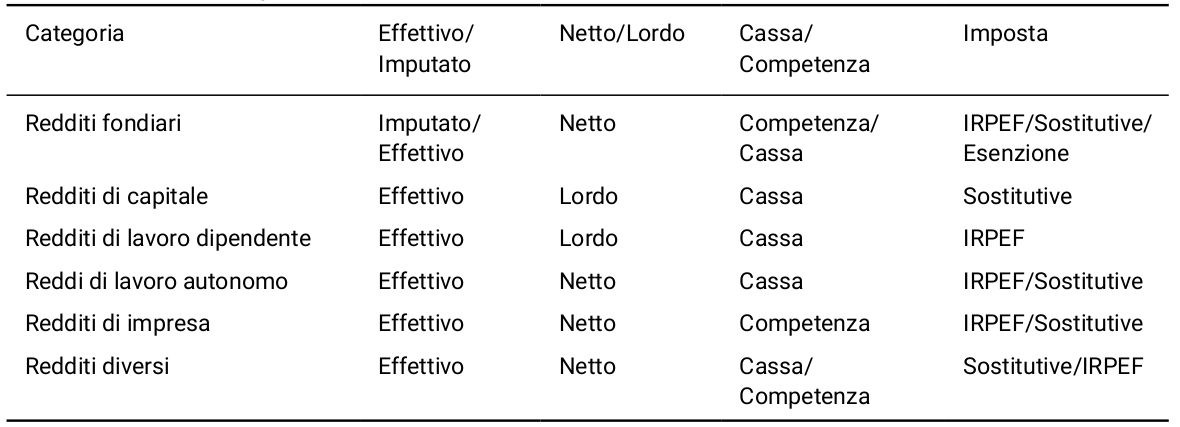
\includegraphics[height=3.8cm]{./figure/categorie-di-reddito-Irpef.png}
\end{figure}


\begin{itemize}
\item È giudizio diffuso tra gli scienziati delle finanze che l'Irpef si sia molto
allontanata dall'idea di tassazione del reddito \alert{complessivo} dell'individuo
prevista dell'impianto originario.
\end{itemize}
\end{frame}

%%%%%%%%%%%%%%%%%%%%%%%%%%%%%%%%%%%%%%%%%%%%
\begin{frame}{Quanto pesano le diverse tipologia di reddito nell'Irpef}
\vspace{-3mm}
\begin{figure}
  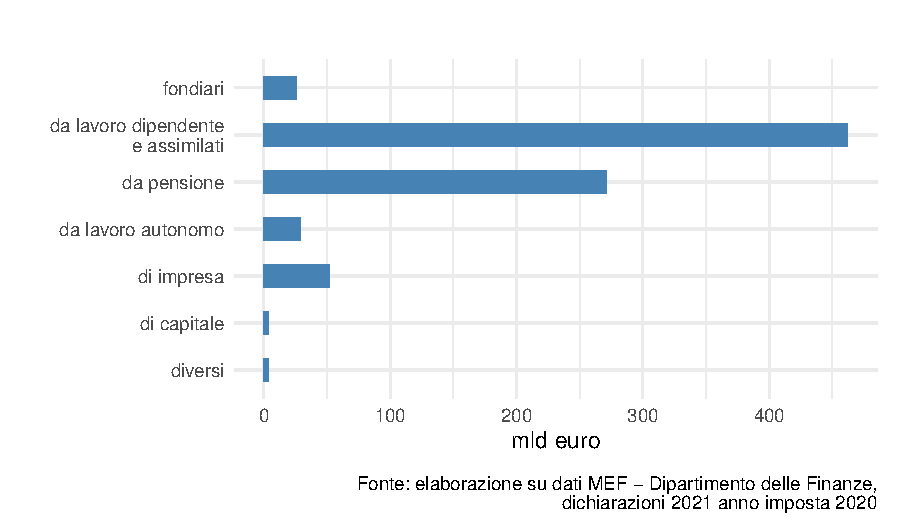
\includegraphics[width=.9\textwidth]{./figure/redditi-dichiarati-per-tipologia-2020-color.pdf}
\end{figure}

\begin{itemize}
\item I redditi di lavoro dipendente e pensioni corrispondeono al 60\% dei redditi
ma "pesano" nel gettito IRPEF per l'86\%
\end{itemize}
\end{frame}

%%%%%%%%%%%%%%%%%%%%%%%%%%%%%%%%%%%%%%%%%%%%
\begin{frame}{Le diverse categorie di contribuenti e il reddito complessivo}
\begin{center}
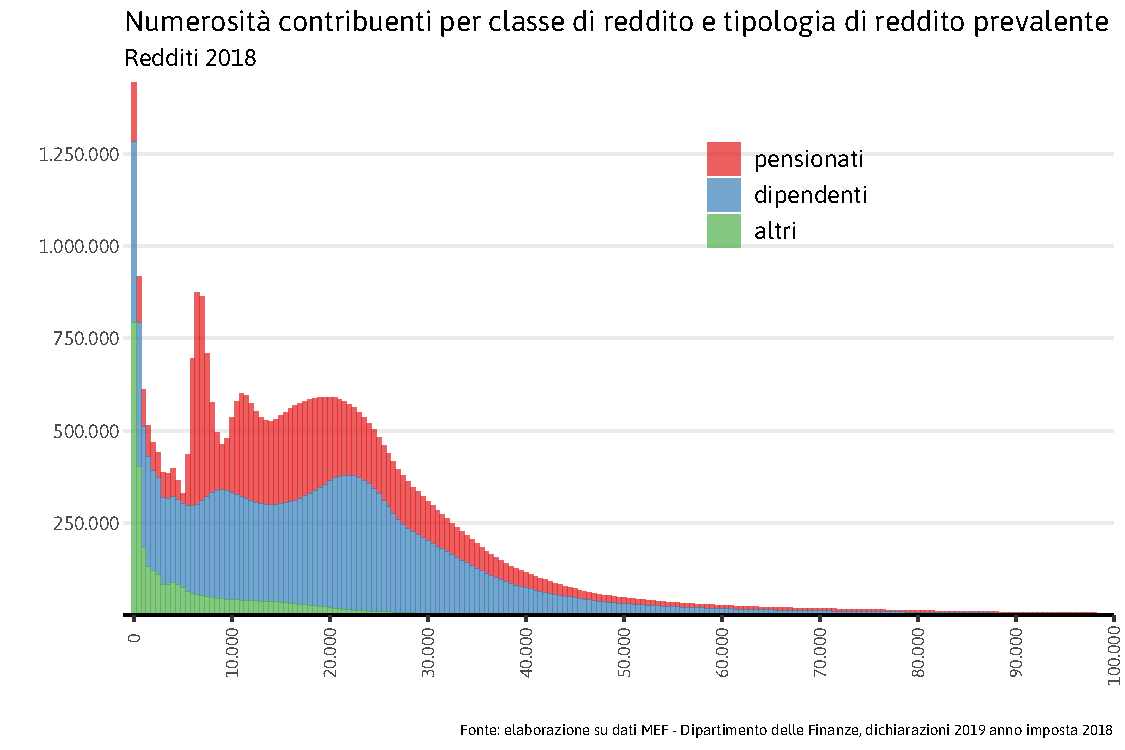
\includegraphics[width=\textwidth]{./figure/distribuzione-classi-irpef.pdf}
\end{center}
\end{frame}

%%%%%%%%%%%%%%%%%%%%%%%%%%%%%%%%%%%%%%%%%%%%
\begin{frame}{Dal reddito complessivo al reddito imponibile}
\small
I casi più rilevanti di \alert{oneri deducibili} sono:
\begin{itemize}
\item contributi previdenziali ed assistenziali obbligatori (versati da lavoratori
autonomi) e contributi facoltativi alla gestione di appartenenza;
\item i contributi versati alle forme pensionistiche complementari (fondi pensione
negoziali, aperti, individuali), per importo massimo di 5.165 €
\item le rendite catastali dell'abitazione principale e degli immobili non locati
(prima del 2012, deduzione limitata alla rendita dell'immobile adibito ad
abitazione principale);
\item contributi e donazioni alle ONG per PVS, per un importo non superiore al 2\%
del reddito complessivo;
\item erogazioni liberali ad istituzioni religiose, non-profit, università, enti
di ricerca;
\item spese mediche ai portatori di handicap;
\item oneri contributivi per domestici e addetti ai servizi personali (``badanti''
e baby-sitter);
\item i contributi a fondi integrativi del sistema sanitario nazionale (SSN); le
donazioni a favore di Onlus (max tra 10\% del RC e 70.000 €)
\end{itemize}
\end{frame}

\section{Detrazioni e personalizzazione dell'imposta}


%%%%%%%%%%%%%%%%%%%%%%%%%%%%%%%%%%%%%%%%%%%%
\begin{frame}{Dall'imponibile all'imposta lorda}

  \begin{columns}
    \begin{column}{.35\textwidth}
\centering
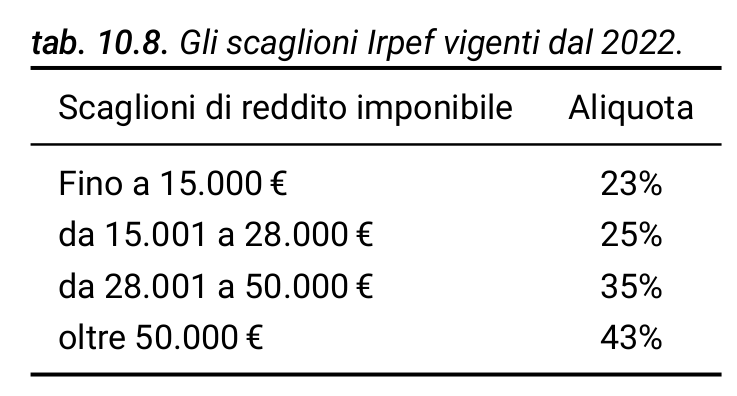
\includegraphics[height=2.7cm]{./figure/scaglioni-IRPEF-2022.png}
\end{column}
\begin{column}{.65\textwidth}
\centering
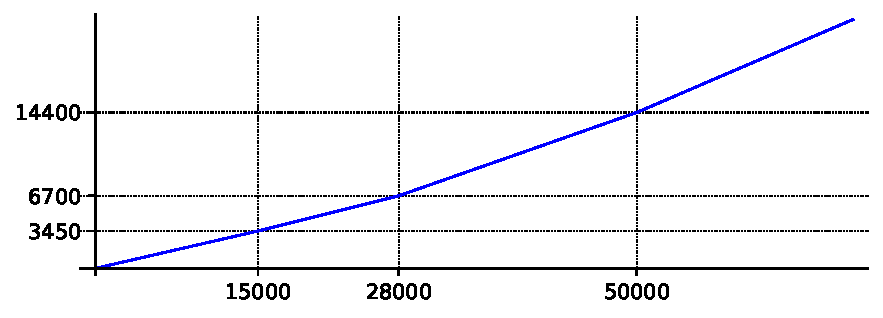
\includegraphics[height=3cm]{./figure/scaglioni-2022-grafico.pdf}
\end{column}
\end{columns}

\small
\begin{tabular}{lll}
Scaglione & Aliquota & Ovvero\\[0pt]
\hline
fino a 15.000 & 23\% & \\[0pt]
da 15.001 a 28.000 & 25\% & $3.450 + 25\% (R - 15.000)$\\[0pt]
da 28.001 a 50.000 & 35\% & $6.700 + 35\% (R - 28.000)$\\[0pt]
da 50.001 & 43\% & $14.400 + 43\% (R - 50.000)$\\[0pt]
\end{tabular}
\end{frame}


%%%%%%%%%%%%%%%%%%%%%%%%%%%%%%%%%%%%%%%%%%%%
\begin{frame}{Le detrazioni}
Una volta determinata l'imposta lorda, si applicano le detrazioni, che possono
essere raggruppate in:
\begin{itemize}
\item Detrazioni \alert{per tipo di reddito} (lavoro dipendente, pensione, autonomo)
\begin{itemize}
\item sono sui redditi da lavoro, al fine di realizzare la discriminazione
qualitativa dei redditi
\item sono maggiori per il lavoro dipendente in ragione del fatto che per tale
reddito è al lordo dei costi di produzione (inoltre consapevolezza della
maggiore evasione sul reddito autonomo)
\end{itemize}
\item Detrazioni \alert{per carichi familiari} (coniuge o figli conviventi \alert{a carico})
\begin{itemize}
\item fiscalmente a carico = reddito $\leq 2840,51€$ (4000 € per figli minori di
24 anni)
\item detrazioni crescenti in base al numero di figli, decrescenti al reddito
(per coniuge: max 800 €, per figli: max 950/1200 €)
\item per figli minorenni, disabili o studenti minori di 21 anni, la detrazione
è stata sostituita dal 2022 dall'\alert{Assegno unico}, con ammontare determinato
in base all'ISEE.
\end{itemize}
\item Detrazioni \alert{per oneri}
\item Detrazioni \alert{per canone di locazione e mutui prima casa}
\item Altre detrazioni con finalità di \alert{incentivazione}
\end{itemize}
\end{frame}
%%%%%%%%%%%%%%%%%%%%%%%%%%%%%%%%%%%%%%%%%%%%
\begin{frame}{Detrazioni, \emph{no tax area} e incapienza}
\begin{itemize}
\item Le detrazioni determinano implicitamente una \alert{no tax area}, un livello di
reddito imponibile al di sotto del quale il contribuente non paga imposta
\begin{itemize}
\item considerando un reddito gravato da un'aliquota $t$, il contribuente
non pagherà imposta se $tR-d\le 0$, ovvero se $R\le d/t$
\item Es. con aliquota del 23\% (primo scaglione) una detrazione fissa di 1.880€
(lavoratore dipendente) determinerebbe una \emph{no tax area} per redditi
inferiori o pari a 1.880€/0.23=8.174€
\item In realtà la detrazione è "a scalare": oltre gli 8000 euro decresce, per
cui la no tax area arriva a 8.145 euro\ldots{}
\end{itemize}
\item Per redditi nella \emph{no tax area}, la detrazione non è goduta per
intero, e ulteriori detrazioni non portano alcun vantaggio al contribuente,
la cui imposta risulta dunque \alert{incapiente} rispetto ad ulteriori benefici
previsti dal sistema fiscale
\item In linea di principio sarebbe possibile superare il problema dell'incapienza
prevedendo un'\alert{imposta negativa}, ovvero l'erogazione di un sussidio pari
all'imposta non goduta (vedi oltre il bonus degli "80 euro")
\end{itemize}
\end{frame}
%%%%%%%%%%%%%%%%%%%%%%%%%%%%%%%%%%%%%%%%%%%%
\begin{frame}{Detrazioni per tipologia di reddito}
\begin{columns}
\begin{column}{.65\columnwidth}
\scriptsize
\begin{tabular}{p{22mm}>{\raggedright}p{48mm}}
  R. imponibile (€) & detrazione (€)\tabularnewline\toprule
   \multicolumn{2}{>{\raggedright}p{60mm}}{\bf Redditi da lavoro dipendente e assimilati}\tabularnewline
  fino a 8.174 & 1.880 (con limite inferiore 690, aumentato a 1.380 se lavoro a tempo determinato) \tabularnewline
  tra 8.175 e 15.000 & 1.880 + Trattamento integrativo di 1.200\tabularnewline
  tra 15.001 e 28.000 & $1.910 + 1.190\times( 28.000 - RD ) / 13.000$ \tabularnewline
  tra 28.001 e 50.000 & $1.910\times(50.000 - RD ) / 22.000$ \tabularnewline
  \multicolumn{2}{>{\raggedright}p{70mm}}{Per i redditi tra 25.000 e 35.000 ulteriore detrazione di 65}\tabularnewline
  \midrule                                           
   \multicolumn{2}{>{\raggedright}p{70mm}}{\bf Redditi da pensione}\tabularnewline
  fino a 8.500 & 1.995 (con limite inferiore 713)\tabularnewline
  tra 8.501 e 28.000 & $700 + 1.225\times( 28.000 - RD ) / 19.500$\tabularnewline
  tra 28.001 e 50.000 & $700\times(50.000 - RD ) / 22.000$ \tabularnewline
  \multicolumn{2}{>{\raggedright}p{70mm}}{Per i redditi non superiori a 29.000 ulteriore detrazione di 50}\tabularnewline
  \midrule                                           
   \multicolumn{2}{>{\raggedright}p{70mm}}{\bf Redditi da lavoro autonomo}\tabularnewline
  fino a 5.500 & 1.265\tabularnewline
  tra 5.501 e 28.000 & $500 + 765\times( 28.000 - RD ) / 22.500$\tabularnewline                      
  tra 28.001 e 50.000 & $500\times(50.000 - RD ) / 22.000$ \tabularnewline
  \multicolumn{2}{>{\raggedright}p{70mm}}{Per i redditi tra 11.000 e 17.000 ulteriore detrazione di 50}\tabularnewline
\bottomrule
\end{tabular}
\end{column}

\begin{column}{.3\columnwidth}
\scriptsize
Il reddito $RD$ è il \alert{reddito per detrazioni}, che si ottiene sommando al reddito complessivo, considerato al netto della rendita catastale per abitazione principale, i redditi da locazioni sottoposti a cedolare secca, i regimi forfetari per lavoratori autonomi e imprese e la deduzione ACE.
\bigskip

La detrazione per redditi da lavoro autonomo è riconosciuta anche per i redditi derivanti da attività commerciali o da lavoro autonomo non esercitati abitualmente e per i redditi di impresa in contabilità semplificata.
\end{column}
\end{columns}
\end{frame}


%%%%%%%%%%%%%%%%%%%%%%%%%%%%%%%%%%%%%%%%%%%%
\begin{frame}{Detrazioni a scalare e aliquote marginali effettive - lavoro dipendente}
\begin{itemize}
\item Le detrazioni per tipologia di reddito "a scalare" modificano l'aliquota
\end{itemize}
marginale effettiva.
\begin{itemize}
\item La situazione precedente il 2022:
\end{itemize}
\begin{figure}
\centering
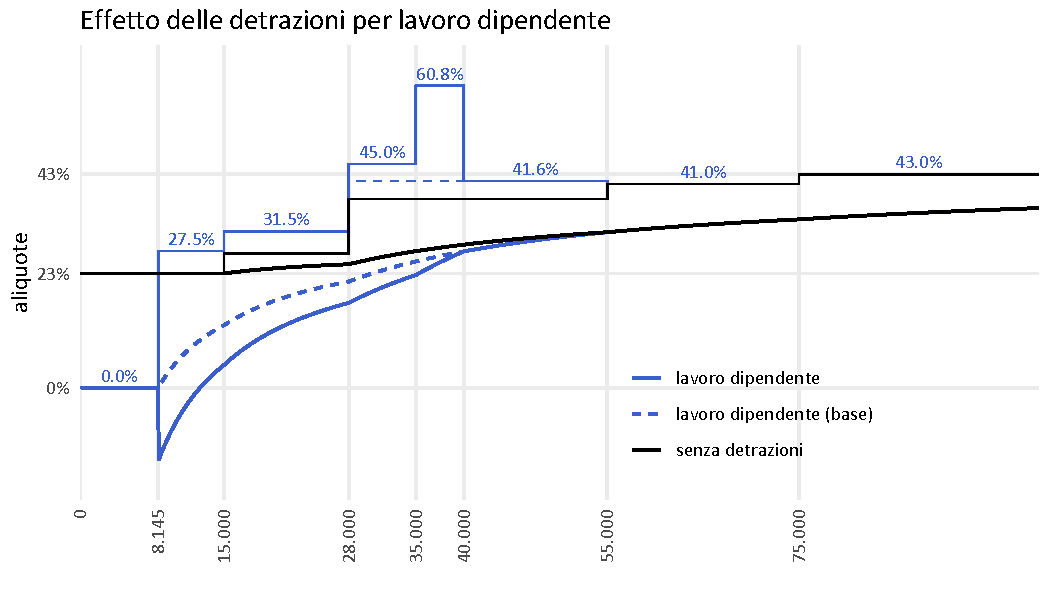
\includegraphics[height=6cm]{./figure/aliquote-medie-marginali-lavoro-dipendente.pdf}
\end{figure}
\end{frame}


%%%%%%%%%%%%%%%%%%%%%%%%%%%%%%%%%%%%%%%%%%%%
\begin{frame}{Detrazioni a scalare e aliquote marginali effettive - confronti}
\begin{columns}
\begin{column}{.33\columnwidth}
\scriptsize
\begin{tabular}{lc}
  \toprule
  Scaglioni & Aliquota\\
  \midrule
  Fino a 15.000\€ &23\%\\
  da 15.001 a 28.000\€ &25\%\\
  da 28.001 a 50.000\€ &35\%\\
  oltre 50.000\€ &43\%\\
  \bottomrule                                                       
\end{tabular}
\end{column}

\begin{column}{.66\columnwidth}
\vspace*{-5mm}
\begin{figure}
\centering
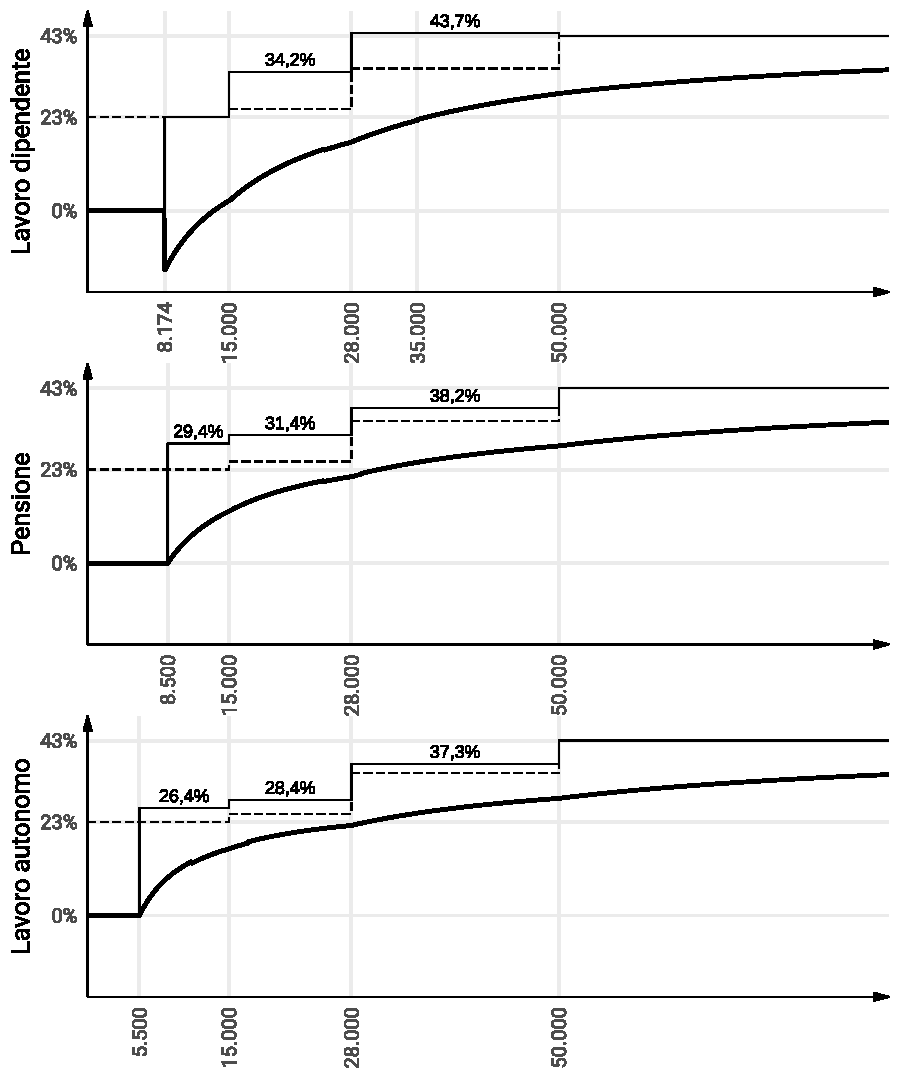
\includegraphics[height=8.5cm]{./figure/aliquote-medie-marginali-2022.pdf}
\end{figure}
\end{column}
\end{columns}
\end{frame}


%%%%%%%%%%%%%%%%%%%%%%%%%%%%%%%%%%%%%%%%%%%%
\begin{frame}{Detrazioni a scalare e aliquote marginali effettive - confronti /2}
\begin{figure}
\centering
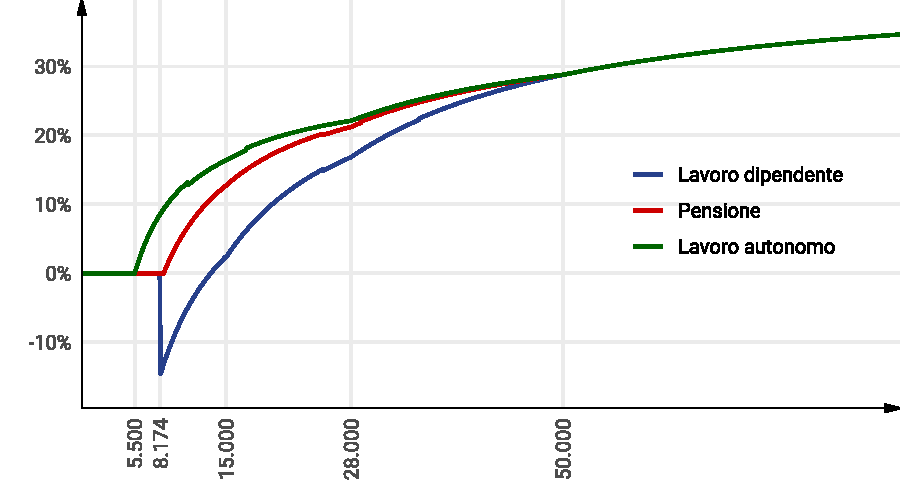
\includegraphics[height=6cm]{./figure/aliquote-medie-2022-color.pdf}
\end{figure}
\end{frame}



%%%%%%%%%%%%%%%%%%%%%%%%%%%%%%%%%%%%%%%%%%%%
\begin{frame}{Detrazioni per carichi di famiglia}
\begin{center}
\begin{tabular}{lrr}
 & detrazione massima & si annulla a\\[0pt]
\hline
Coniuge & 800 & 80.000\\[0pt]
Figlio fino a 3 anni & 1.220 & 95.000\\[0pt]
Figlio $>$ 3 anni & 950 & 95.000\\[0pt]
Altri familiari & 750 & 80.000\\[0pt]
\end{tabular}
\end{center}

\begin{itemize}
\item Se più figli, il limite di 95.000 è aumentato di 15.000 per ciascun figlio
oltre il primo (N.B. si considera il "reddito per detrazioni")
\item Per figli portatori di handicap, detrazione aumentata di 400
\item Se più di 3 figli, la detrazione è aumentata di 200 per ciascun figlio
\item Se 4 figli o più, detrazione fissa aggiuntiva di 1200 euro (riconosciuta
come credito di imposta in casi di incapienza). Dunque, se 4 figli di cui 2 sotto i 3 anni:
$[2\times(950+200)+2\times(1.220+200)](140.000-R)/140.000+1200$
\item Ripartita tra entrambi i genitori se il coniuge non è a carico
\item Come la detrazione per reddito, l'aliquota "a scalare" comporta un aumento
dell'aliquota marginale implicita
\end{itemize}
\end{frame}

%%%%%%%%%%%%%%%%%%%%%%%%%%%%%%%%%%%%%%%%%%%%
\begin{frame}{Le detrazioni per oneri (\emph{tax expenditures})}
\begin{itemize}
\item A fronte di specifiche categorie di spesa sono previste detrazioni nella
misura del 19\% o 24\% della spesa stessa (in alcuni casi franchigie e tetti
massimi)
\item Sono finalizzate a
\begin{itemize}
\item personalizzare il tributo in relazione a circostanze personali che
incidono sulla capacità contributiva (esempio: spese mediche, spese
funebri, premi assicurazione vita)
\item incentivare impieghi "meritori" del reddito (frequenza corsi universitari,
spese sportive per i ragazzi)
\end{itemize}
\item Quasi tutte al 19\%, al 24\% le erogazioni liberali a favore di Onlus e
partiti/movimenti politici
\item Dal 2020, con alcune eccezioni (spese sanitarie ed erogazioni liberali), la
detraibilità non è ammessa per redditi superiori a 240.000, ed è ammessa in
misura parziale per redditi tra 120.000 e 240.000
\end{itemize}
\end{frame}

%%%%%%%%%%%%%%%%%%%%%%%%%%%%%%%%%%%%%%%%%%%%
\begin{frame}{Detrazioni per oneri}
\begin{figure}
\centering
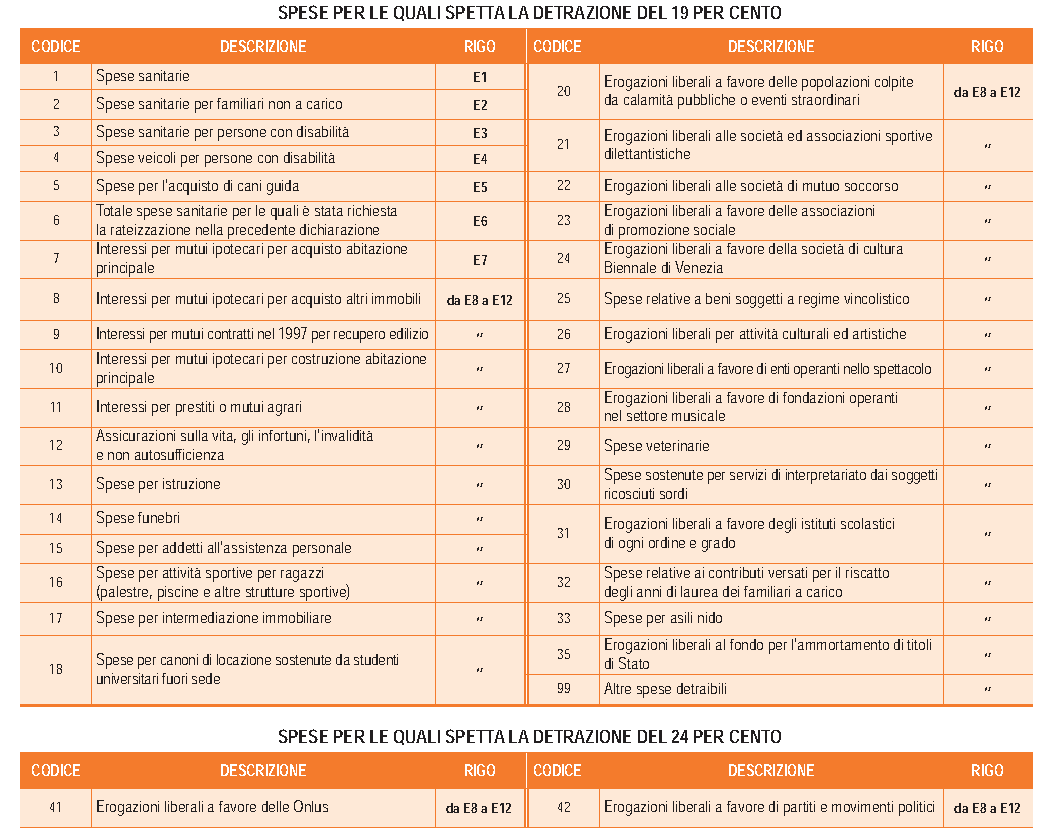
\includegraphics[height=8cm]{./figure/oneri-detrazioni-2014.pdf}
\end{figure}
\end{frame}

%%%%%%%%%%%%%%%%%%%%%%%%%%%%%%%%%%%%%%%%%%%%
\begin{frame}{Altre detrazioni}
\begin{itemize}
\item Detrazione degli interessi su mutui contratti per l'\emph{acquisto} della prima
casa (19\% entro limite 4.000 euro) e della sua \emph{costruzione} (19\% entro
limite 2.582,28)
\item Detrazione (minima!) sul canone di locazione, variabile a seconda del
reddito e a seconda del fatto che il canone sia libero o "convenzionale"
\begin{itemize}
\item canone libero: 300 se reddito inferiore a 15.493,71, 150 se reddito
inferiore a 30.987,41
\item canone convenzionale: 495,80 se reddito inferiore a 15.493,71, 247,90 se
reddito inferiore a 30.987,41
\end{itemize}
\item Detrazioni, speciali e temporanee, per interventi di recupero del patrimonio
edilizio, interventi di risparmio energetico, ecc. rateizzate in 5-10 anni
\end{itemize}
\end{frame}

%%%%%%%%%%%%%%%%%%%%%%%%%%%%%%%%%%%%%%%%%%%%
\begin{frame}{Effetti redistributivi dell'Irpef sui redditi individuali}
\begin{figure}
\centering
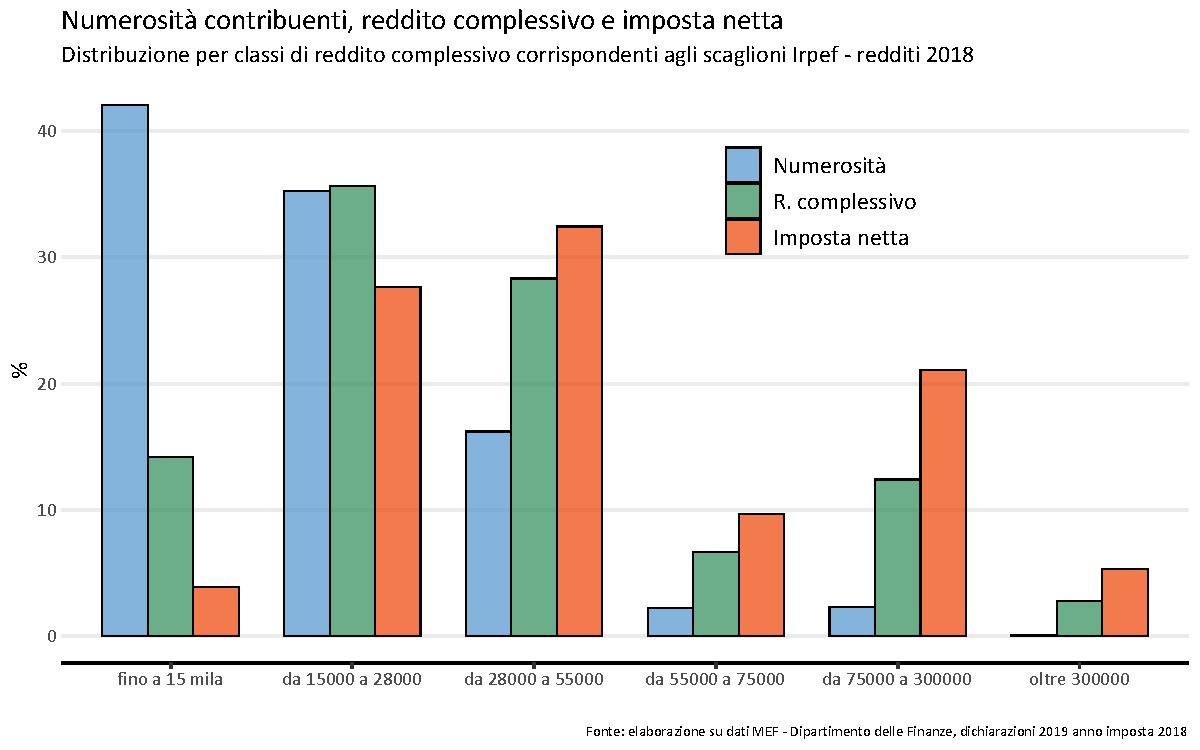
\includegraphics[width=\textwidth]{./figure/irpef-classi-reddito-imposta-aggregato.pdf}
\end{figure}
\end{frame}

%%%%%%%%%%%%%%%%%%%%%%%%%%%%%%%%%%%%%%%%%%%%
\begin{frame}{Effetti redistributivi dell'Irpef sui redditi familiari}
\begin{figure}
\centering
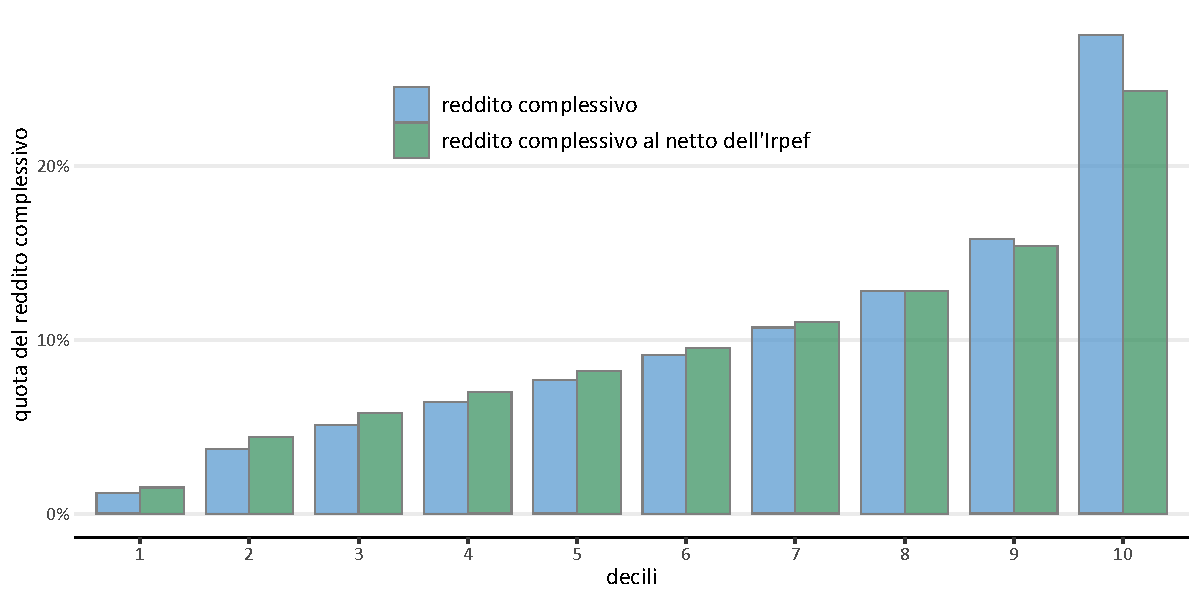
\includegraphics[width=\textwidth]{./figure/effetti-redistributivi-irpef.pdf}
\end{figure}

\tiny Fonte: elaborazione su dati Bosi-Guerra, 2020, p. 148
\end{frame}

\end{document}